%% Copernicus Publications Manuscript Preparation Template for LaTeX Submissions
%% ---------------------------------
%% This template should be used for copernicus.cls
%% The class file and some style files are bundled in the Copernicus Latex Package, which can be downloaded from the different journal webpages.
%% For further assistance please contact Copernicus Publications at: production@copernicus.org
%% https://publications.copernicus.org/for_authors/manuscript_preparation.html

%% Please use the following documentclass and journal abbreviations for preprints and final revised papers.

%% 2-column papers and preprints

\documentclass[gmd, manuscript]{copernicus}
%% \usepackage commands included in the copernicus.cls:
%\usepackage[german, english]{babel}
%\usepackage{tabularx}
%\usepackage{cancel}
%\usepackage{multirow}
%\usepackage{supertabular}
%\usepackage{algorithmic}
%\usepackage{algorithm}
%\usepackage{amsthm}
%\usepackage{float}
\usepackage{graphicx}
\usepackage{caption}
%\usepackage{subfig}
\usepackage{subfigure}
\usepackage{hyperref}
%\usepackage{rotating}
\usepackage{subcaption}
\usepackage{enumitem}
\usepackage{booktabs}
\usepackage{ulem}
\usepackage{makecell}

\setlist[itemize,1]{label=\Large\textbullet}
\usepackage[utf8]{inputenc}
\usepackage[table,xcdraw,svgnames]{xcolor}  % svgnames adds named colors
\usepackage[table]{xcolor}                   % basic table colors
%\captionsetup[sub]{labelformat=simple, labelsep=colon}
%\renewcommand{\thesubtable}{(\alph{subtable})}

\newcommand{\alphcaption}[1]{%
    \stepcounter{enumi}%
    \textbf{(\alph{enumi}) #1}%
}

\definecolor{B}{HTML}{006EB8}

\begin{document}
\title{TOAR-classifier v2: A data-driven classification tool for global air quality stations}
% \Author[affil]{given_name}{surname}
\Author[1,*][k.mache@fz-juelich.de]{Ramiyou Karim}{Mache} %% correspondence author
\Author[1]{Sabine}{Schröder}
\Author[1,*]{Michael}{Langguth}
\Author[1]{Ankit}{Patnala}
\Author[1,2]{Martin G.}{Schultz}

\affil[1]{Jülich Supercomputing Centre, Forschungszentrum Jülich, 52425 Jülich, Germany}
\affil[2]{Department of Mathematics and Computer Science, University of Cologne, Cologne, Germany}
\affil[*]{no longer at institute}
%\affil[]{ADDRESS}

\runningtitle{ML based station classification}
\runningauthor{Ramiyou Karim Mache}

\received{}
\pubdiscuss{} %% only important for two-stage journals
\revised{}
\accepted{}
\published{}
%% These dates will be inserted by Copernicus Publications during the typesetting process.

\firstpage{1}

\maketitle

\begin{abstract}
Accurate characterization of station locations is crucial for reliable air quality assessments such as the Tropospheric Ozone Assessment Report (TOAR). While urban and rural areas are relatively well-defined, the boundaries and identity of suburban areas remain ambiguous, overlapping with both urban and rural zones and varying due to cultural and social factors. This study investigates a machine learning approach to classify 24,348 stations in the unique global TOAR database as urban, suburban, or rural. We tested two different  methods: unsupervised K-means clustering with three clusters, and an ensemble of supervised learning classifiers including random forest, CatBoost, and LightGBM. We  integrate these classifiers into a robust voting model, leveraging their collective predictive power. To address the inherent ambiguity of suburban areas, we implement a grid-search adjusted threshold probability technique. Our models, trained on the TOAR station metadata, are evaluated on 1,979 unseen data points. K-means clustering achieves 71.88 \% and 87.67\% accuracy for urban and rural areas respectively, but only 15.84\% for suburban zones. The supervised classifiers surpass this performance, reaching over 84\% accuracy for urban and rural categories, and 66\% - 72\% for suburban areas. The adjusted threshold technique significantly enhances overall model accuracy, particularly for suburban classification. The good separation of our model is confirmed through evaluation with NOx and PM2.5 concentration measurements, which were not included in the training data. Furthermore, manual inspection of 30 randomly selected sites with Google maps reveals that our method provides a better label for the station type than the labels that were reported by data providers and used in the model evaluation. The objective station classification proposed in this paper therefore provides a robust foundation for type-of-area-specific air quality assessments in TOAR and elsewhere.
%In this study, we introduce an advanced and unbiased machine learning classifier designed to categorize station locations within the Tropospheric Ozone Assessment Report (TOAR) database. We trained various machine learning models on TOAR metadata to classify station locations as urban, suburban, or rural. Our methodology includes exploring different models: unsupervised K-means clustering with three clusters, and popular supervised learning classifiers such as random forest, CatBoost, and LightGBM. Furthermore, we integrate these supervised classifiers into a robust voting model for enhanced performance. Recognizing the subjective nature of defining suburban areas, we adjust our classification based on a threshold probability for different classes, which significantly enhances the overall accuracy and accuracy of classifying suburban locations. We assess our machine learning methods on a test set of 1000 unseen data points using classification metrics like accuracy and confusion matrices. Additionally, we employ the Adjusted Rand Index (ARI) and Normalized Mutual Information (NMI) to further evaluate the quality of the K-means clusters. For supervised learning, we also evaluate the primary air pollutant concentrations of NO$_x$ and PM2.5, which were not included during the training phase. The K-means clustering analysis, when applied to 1000 previously unseen data points in our test set, reveals distinct separation between clusters and substantial distances between centroids. This separation is quantitatively supported by the Adjusted Rand Index (ARI) and Normalized Mutual Information (NMI) scores of 0.3 and 0.31, respectively. A detailed examination of the clusters demonstrates strong performance in identifying urban and rural areas, with accuracy rates of 71\% and 69\% respectively. However, the model struggles with suburban classification, achieving only 23\% accuracy for this category. The supervised classifiers demonstrate comparable performance when tested on 1000 previously unseen data points, achieving overall accuracy rates exceeding 79\%. A detailed analysis of these models' performance across different categories reveals high accuracy in classifying urban and rural areas, with each category surpassing 84\% accuracy. However, the suburban category proves more challenging, with accuracy rates falling between 63\% and 65\%. Our innovative adjusted threshold probability technique substantially enhances the accuracy of these supervised machine learning models. Additionally, box plot analysis of the 75th percentile of primary air pollutants, including NOx and PM2.5, indicates a clear distinction between urban, suburban, and rural areas.

%In this paper, we propose an advanced and unbiased machine learning classifier to characterize station locations in the Tropospheric Ozone Assessment Report (TOAR) database. We trained machine learning models on TOAR metadata to classify station locations as urban, suburban, or rural. Our approach explores different models: unsupervised K-means clustering with three clusters, and popular supervised learning classifiers including random forest, CatBoost, and LightGBM. Additionally, we combine these supervised classifiers into a robust voting model for this task. Given the subjective nature of defining suburban areas, we adjust our classification based on a threshold probability for different classes. This adjustment significantly improves the overall accuracy and the accuracy of classifying suburban locations. We evaluate our machine learning methods on a test set of 1000 unseen data points using classification metrics such as accuracy, and confusion matrices. We also used the Adjusted Rand Index (ARI), and Normalized Mutual Information (NMI) to further evaluate the quality of K-means clusters. Additionally, for supervised learning, we evaluated the air primary pollutant concentrations of NO$_x$ and PM2.5, which were not used during the training phase. 
\end{abstract}
%\copyrightstatement{TEXT} %% This section is optional and can be used for copyright transfers.
%\newpage

\section{Introduction} 
Ozone in the troposphere plays a crucial role in human and environmental health, \citep{post2012variation, griffiths2021tropospheric}. As a significant atmospheric pollutant and greenhouse gas, ozone profoundly impacts air quality and contributes to the dynamics of climate change  \citep{madronich2023changes, orru2013impact}.
Accurate ozone monitoring data is essential for shaping public health policies and ecological regulations. Modern data infrastructures can be used to provide atmospheric scientists with the necessary metrics to quantify ozone's impact on climate, human health, and vegetation \citep{gaudel2018tropospheric, flemingchapter, mills2018nitrogen, teakles2017impacts, cooper2014global, monks2015tropospheric, schultz2015global}. 
% [mgs] I mention these three because they are the TOAR topics
%Accessing ozone data presents challenges including limited availability, concerns about data quality, the need for technical expertise, and restrictions imposed by data access policies, necessitating collaborative efforts to improve accessibility and promote informed decision-making. 
In 2021, the International Global Atmospheric Chemistry project (IGAC) launched the second phase of the Tropospheric Ozone Assessment Report (TOAR-II) to undertake a comprehensive review of the global distribution and trends of tropospheric ozone. A key accomplishment of TOAR-II is the development of a new terabyte-scale relational database of surface ozone observations and related variables. This database includes hourly measurement data and enriched metadata from 1970 to 2023, collating information from over 20,000 measurement sites worldwide through collaboration among multiple data centers and individual researchers (Schröder et al., manuscript in preparation). The new TOAR-II database replaces and extends the first TOAR database that has been described in \cite{schultz2017tropospheric}. 
%Ozone concentrations vary strongly across different regions and concentration patterns differ across pollution regimes. 
Ozone levels exhibit significant regional variations and distinct patterns across different pollution environments. For example, urban environments with large ozone precursor emissions can exhibit "zero ozone" (i.e., ozone at sub-nmol fractions) situations and very large variability, while concentrations in rural areas tend to be smoother \citep{zhou2022spatiotemporal, Schultz2017}. To accurately assess the ozone situation at individual locations and interpret ozone trends across the globe, it is therefore important to characterize measurement sites in a globally consistent and objective manner. While many measurement networks provide information about the station location or "type of station" and "type of station area", %\textcolor{red}{almost 10000 out of 24000 stations have no label and classify as unknowns, see Figure~\ref{data_dist_a}. In addition} 
this metadata information is inconsistent between regions and error-prone as it involves some subjective judgement \citep[c.f.,][]{tapia2016new}. 

%\textcolor{B}{Inconsistency claim (L36/37). You state that TOAR labels are inconsistent/error-prone. Please provide a reference or a concrete rationale/example for this statement. (You later discuss misalignment; connect those to this claim.)} \textcolor{red}{We should discuss this!}

In the first assessment of TOAR \cite{schultz2017tropospheric} pioneered a new way to classify stations in a globally uniform way based on a set of Earth Observation (EO) datasets that have been processed at the station locations. This method used manually selected threshold values of station altitude, population density, nighttime light intensity, NO$_2$ column density, and NOx emissions to characterize stations as urban or rural. While this approach provided a useful distinction between "clearly urban" and "clearly rural" sites, it fell short of classifying all sites as almost half of the stations remained unclassified, see Figure~\ref{data_dist}. Furthermore, the method was criticized for lack of an objective definition of the threshold values. Especially, the boundaries and characteristics of suburban areas remain ambiguous. Suburban zones, typically located at the periphery of cities and noted for lower density and residential land use, often overlap with both urban and rural regions. Their definition is shaped by cultural, social, and psychological factors, resulting in varied interpretations and a lack of universal consensus, \citep{hesse2018suburbanisation, airgood2019defining}. This emphasizes the need for an objective and automated station classification method. In this study, we propose a new machine learning (ML) approach to develop a more advanced and unbiased classifier using similar objective metadata from the TOAR-II database. Our primary objective is to create a machine learning model that classifies stations in the TOAR database as urban, suburban, or rural.
%In this study, we propose a new machine learning approach to develop a more advanced unbiased classifier using metadata. Our main task is to build a machine learning model to classify stations ('type\_of\_area' in the TOAR database) as urban, suburban, or rural.
% [mgs] The following is still a bit unclear - almost there, but try to be a bit more explicit
We implement and compare two methodologies: unsupervised learning using K-means clustering, %where all station characteristics are treated as unknown, 
and supervised learning classifiers such as random forest, CatBoosting, and LightGBM. In supervised learning, a subset of station characteristics is known and used to train the classifiers which are then used to predict the class of unlabeled  stations. The supervised models are evaluated individually and after applying a robust voting method. Furthermore, an adjusted threshold technique is applied to enhance the identification of suburban stations. The remainder of this paper is organized as follows: Section 2 describes the data and methods used, Section 3 presents the results and discussion, and a general conclusion wraps up the paper.
%The next section presents \sout{the} data and \textcolor{red}{methods} \sout{methodology}, followed by Section \ref{results_discusion}, which focuses on the results and discussion. A general conclusion wraps up the paper.
%\textcolor{B}{In the Introduction, when outlining the problem and motivating the study in the last paragraph, consider mentioning that almost 10,000 of the 24,000 stations have no label, which calls for an automated approach.} \textcolor{red}{already in the text, I add ref}

\section{Data and methods}\label{data_method}
This section provides an overview of our data sources, machine methods used, and evaluation metrics. We begin by introducing the TOAR-II database and the station metadata that are used as inputs of the ML models. We then detail our data preparation process, including preprocessing, feature engineering, and feature selection, all critical steps in preparing data for ML models. Finally, we present a concise summary of the ML models employed in this study and the evaluation metrics used to assess their performance.

%In this section, we provide a brief introduction to the TOAR database and the station metadata from Earth Observations (EO). We outline the data preprocessing, feature engineering, and feature selection processes, which are essential for preparing data for machine learning models. Additionally, we offer an overview of the machine learning models employed in this study and the evaluation metrics used to assess their performance.

%In this section, we briefly introduce the TOAR database and the station metadata from EO. We describe  the data prepossessing, feature engineering, and feature selection, all crucial steps in preparing data for machine learning models. Additionally, we provide a brief overview of the machine learning models utilized in this work, 
%% [mgs] don't repeat model list: including K-means clustering, random forest, CatBoosting, and LGBM, 
%along with the evaluation metrics used to measure the performance of our models.

\subsection{TOAR-II database and station metadata}
Developed in the context of TOAR phase II, the TOAR-II database stands as one of the world's largest collections of near-surface ozone measurements and related information. The database can be accessed through web services which provide a comprehensive suite of ozone-related data products including standard statistics, health and vegetation impact metrics, and trend information (\href{https://toar-data.fz-juelich.de/}{https://toar-data.fz-juelich.de/}). The TOAR-II database includes extensive information describing the locations of air quality measurement stations based on pollution-relevant properties. These properties are extracted from EO data and stored as station metadata in the database. This metadata offers contextual information about the measurement site, enabling station location characterization. Table~\ref{meta_variables} below summarizes all metadata used in this study including references to the data origin.
\begin{table}[htb!]
\caption{Station metadata in the TOAR database used in this work.}
%s\vspace{0.cm}
\centering
\resizebox{0.91\columnwidth}{!}{%
\begin{tabular}{|l|l|l|}
\hline
\textbf{Variable name}  & \textbf{Description}     & \textbf{Type} \\ \hline
lon, lat & \begin{tabular}[c]{@{}l@{}}longitude,  latitude represent the geographical coordinates of station. \\ We did not use these coordinates as predictors in  the machine learning model\end{tabular}  & Numeric   \\ \hline

area\_code  & Unique code of the station in TOAR database & String      \\ \hline
altitude & altitude of the station location in meter (m)  & Numeric       \\ \hline
\begin{tabular}[c]{@{}l@{}}mean\_topography\_srtm\_alt\_90m\_year1994\\ mean\_topography\_srtm\_alt\_1km\_year1994\end{tabular}    & \begin{tabular}[c]{@{}l@{}} mean value within 90m and 1km of relative altitude of the year 1994.\\ data source: NASA Shuttle Radar Topographic Mission (SRTM) \citep{jarvis2008hole} \end{tabular}  & Numeric       \\ \hline
\begin{tabular}[c]{@{}l@{}}max\_topography\_srtm\_relative\_alt\_5km\_year1994 \\ min\_topography\_srtm\_relative\_alt\_5km\_year1994 \\ stddev\_topography\_srtm\_relative\_alt\_5km\_year1994\end{tabular}  & \begin{tabular}[c]{@{}l@{}} maximum, minimum, and standard deviation of the \\relative altitude within a radius of 5km around the station in 1994 \\ data source: NASA Shuttle Radar Topographic Mission (SRTM) \citep{jarvis2008hole}  \end{tabular} & Numeric       \\ \hline
climatic\_zone\_year2016 & \begin{tabular}[c]{@{}l@{}}climate zone of the year 2016. Provides information about climatic conditions\\ at a location including whether it tends to be hot or cold, humid or dry, \\ or exhibits a tropical climate \\ data source:  University of East Anglia Climatic Research Unit \citep{harris2017university} \end{tabular}    & Category      \\ \hline
\begin{tabular}[c]{@{}l@{}}mean\_stable\_nightlights\_1km\_year2013\\ mean\_stable\_nightlights\_5km\_year2013\\ max\_stable\_nightlights\_25km\_year2013\\ max\_stable\_nightlights\_25km\_year1992\end{tabular}   & \begin{tabular}[c]{@{}l@{}}average and maximum nighttime light value of the years 1992, and 2013\\in 1km, 5km, and 25km around the station location. The values in this data set \\ represent a  brightness index ranging from 0 to 63.\\
data source: NOAA National Centers for Environmental Information (NCEI) \citep{kroehl1982national}\end{tabular} & Numeric       \\ \hline
\begin{tabular}[c]{@{}l@{}}mean\_population\_density\_250m\_year2015      \\ mean\_population\_density\_5km\_year2015 \\ max\_population\_density\_25km\_year2015\\ mean\_population\_density\_250m\_year1990\\ mean\_population\_density\_5km\_year1990  \\ max\_population\_density\_25km\_year1990\end{tabular} & \begin{tabular}[c]{@{}l@{}}Average and maximum population density of the years 1990, and 2015 \\in 250m, 5km, and 25km radius around the station location \\
data source: The European Commission, Joint Research Centre, \citep{florczyk2019ghsl} \end{tabular} & Numeric       \\ \hline
\begin{tabular}[c]{@{}l@{}}mean\_nox\_emissions\_10km\_year2015\\ mean\_nox\_emissions\_10km\_year2000\end{tabular}  & \begin{tabular}[c]{@{}l@{}}Average annual NOx emission of the years  2000 and 2015 in a 10km radius around \\ the station location
\\data source: Copernicus Atmosphere Monitoring Service \citep{granier2019copernicus}\end{tabular} & Numeric \\ \hline
timezone  & Geographical area, such as Africa, America, Europe, etc. & Category      \\ \hline
type\_of\_area (target)& \begin{tabular}[c]{@{}l@{}}Characterization of station location (urban, suburban, rural, or unknown) reported \\by the data providers of the TOAR database. This variable is not used in K-means clustering,\\ and the known part, i.e stations labelled as urban, suburban, rural, \\  are employed to train supervised classifiers.\end{tabular}  & Category      \\ \hline
\end{tabular}%
}
\label{meta_variables}
\end{table}

Some metadata, such as station coordinates, are provided by many air quality agencies and scientific institutions that contribute to the TOAR database. The other metadata elements listed in Table~\ref{meta_variables} stem from  EO datasets, which were downloaded from the respective provider sites. A special web service called Geospatial point extraction and aggregation service (GeoPEAS) has been developed to compute the aggregate information from the original gridded products. More information about the EO datasets used in GeoPEAS can be found on \href{https://toar-data.fz-juelich.de/api/v2/#stationmeta}{https://toar-data.fz-juelich.de/api/v2/\#stationmeta}.
%{\bf MISSING HERE is a short description of the EO datasets as in GeoPEAS!!!}
%{\bf sschr: Information about the EO datasets used in GeoPEAS can be found here: https://toar-data.fz-juelich.de/api/v2/#stationmeta}
After the metadata extraction with GeoPEAS, all metadata are available as lists of key-value pairs with the keys corresponding to the variable names in Table~\ref{meta_variables}. 
For further processing, this data was collected into one table with the keys as data columns and the individual stations as rows.

%\textcolor{B}{Section 2.2: Provide information on the distribution of TOAR labels in the dataset. How many cases are in the suburban class? Are the class distributions approximately balanced?}

%\textcolor{B}{L95–99: This is a very important paragraph, as it addresses the reliability of the TOAR labels. Please report explicitly the level of agreement between TOAR labels and the manual approach. What was the distribution of labels in each classification approach, and how often did the suburban category agree/disagree? Did one or several of the authors (independently?) perform the manual classification? This information is crucial to assess the reliability of the reference labels. What do you mean by “clear decision boundaries”? Did you pick particularly easy stations for the manual labeling exercise? Is the proportion of agreement between TOAR labels and manual labels higher than for the 25 worst predictions (Table 6) (if I counted correctly, 8 out of 25 agree)?}

\subsection{Data preprocessing and feature selection}
%% [mgs] We must discuss with Sabine when we will have an update of the EO metadata extraction -- there should be no more/much less missing values after reprocessing!!
The first step in our data preprocessing pipeline consists of cleaning the dataset. This involves removing all duplicate data points, replacing values of -999.0 with NaN to denote missing values, and eliminating rows where all metadata information is missing. To ensure consistency, we filtered out rows with inconsistent values, such as negative population density or negative maximum stable lights. In total, this step eliminates 211 stations out of 24,348 stations.
%% This is important information: where does this come from?? Shouldn't appear in the database!!!
For handling missing altitude data, we fill these with mean\_topography\_srtm\_alt\_90m\_year1994. Other numerical missing values are estimated using the regression iterative imputer, \cite{rubinsteynfancyimpute}, and categorical missing values fill with most frequent instance. 
Categorical variables are encoded using OneHotEncoder from scikit-learn, \cite{pedregosa2011scikit}. %\textcolor{red}{\sout{Additionally, we applied a Box-Cox transformation to the NOx emissions data to normalize its distribution.}}

%\textcolor{red}{For K-means clustering, we preprocess numerical features by standard scaling and IQR-based (Q1 − 1.5·IQR, Q3 + 1.5·IQR) outlier clipping, steps critical for this algorithm due to its reliance on Euclidean distance and sensitivity to feature scale and outlier-driven centroid shift.} 
For K-means clustering, numerical features were scaled using standard scaling, and outliers were handled with IQR-based clipping within the range [Q1 − 1.5·IQR, Q3 + 1.5·IQR], where IQR (Interquartile Range) is the difference between the third quartile (Q3) and the first quartile (Q1). These preprocessing steps are essential to mitigate the algorithm’s sensitivity to feature scale and outliers. For supervised learning algorithms, we applied a robust scaler, \cite{pedregosa2011scikit} to the entire dataset, which proved more effective for this task compared to alternative scaling methods such as standard or min-max scaling. This scaling approach helps mitigate the impact of outliers and ensures consistent feature ranges. In the feature selection process, we prioritized variables containing the most recent available information, ensuring our model utilizes the most up-to-date data for classification.
%\textcolor{B}{L88: Check the numbers. If you remove 1,000 cases, you should end up with 21,378, I believe.}
%The entire dataset is then scaled using a robust scaler \cite{???}, which provides superior results for this task compared to other scaling options, such as the standard and min-max scaler. For feature selection, we prioritize variables with the most recent information available.
%% In the description of the data above, the text should explicitly state that some of the EO datasets are available for several years!
Notably, geographical coordinates (longitude-latitude) and station codes are excluded from the machine learning models to prevent overfitting to geolocation.
%% perhaps cite Hanna Meyer (Uni Münster) -- I believe she published a paper on this
%% [mgs]: this is a discussion - that doesn't belong here yet: In supervised learning, mean\_topography\_srtm\_alt\_90m\_year1994 yields the highest accuracy instead of altitude. 
Following preprocessing steps,  the final dataset comprises 24,125 stations. Of these, 13,225 are labeled as urban, suburban, or rural, while the remaining 10,900 are unlabeled. The distribution of the processed data is presented in Figure \ref{data_dist}. 
%\textcolor{red}{\sout{After preprocessing, the dataset consists of 22,378 rows, from which, 10,900 stations are unlabeled and only 13,225 are labeled as urban, suburban or rural. The distribution of the processed dataset is shown on Figure \ref{data_dist_a}.}} % {\bf ???}
%[mgs] original wording was: data points. 
%For K-means clustering, we utilize 21351 data points for training and 1000 data points for testing. 

For the K-means clustering analysis, we allocated 22,111 samples for model training and reserved 15\% of the labeled data (1,979 samples) for testing.
The supervised models were trained on a smaller subset because only 13,225 stations were explicitly classified as urban, suburban, or rural by the TOAR data providers. The remaining 10,900 stations lacked this specific classification, being reported as 'unknown' or without a designated category. %(\textcolor{red}{move this sentence to introduction?}). 
%In the supervised learning approach, only 12,453 stations are characterized as urban, suburban, or rural, while 9,898 remain unknown i.e. not reported as urban, suburban, or rural by the TOAR data provider. 
%% [mgs] This requires more explanation: why are they unknown? How does this work? It is probably better to write this AFTER you describe the methods. Perhaps as another subsection "Resulting dataset" or something similar?? Add a bit more information on how these >20,000 and 11, xxx stations are distributed and where their data comes from; i.e. add some description of what the reader sees in Figure 1.
%For the supervised models, 
We used 85\% of the labeled data (11,211  samples) for training while the remaining 15\% is allocated for testing. The distribution of training and testing datasets is presented in Figure \ref{data_dist}. As shown, the training dataset is imbalanced, with a higher number of urban stations compared to suburban and rural ones. However, the class imbalance is not severe. We address it by applying the Synthetic Minority Oversampling Technique (SMOTE) \citep{chawla2002smote} to the training data before fitting the supervised classifiers. It is important to note that SMOTE was applied exclusively to the training set and not to the test data. 
The trained classifier is then used to predict the characteristics of unlabeled stations as illustrated in Figure~\ref{data_split}.

%\textcolor{B}{L88–94: You have 12,408 stations with labels, but you cluster and predict the entire dataset of 22,378 stations. What is being done with the 10,000 stations that have no label? Is the predicted classification of these stations used for something in the manuscript? Please make this more obvious.}\textcolor{red}{Done!}

\begin{figure}[htb!]
    \centering
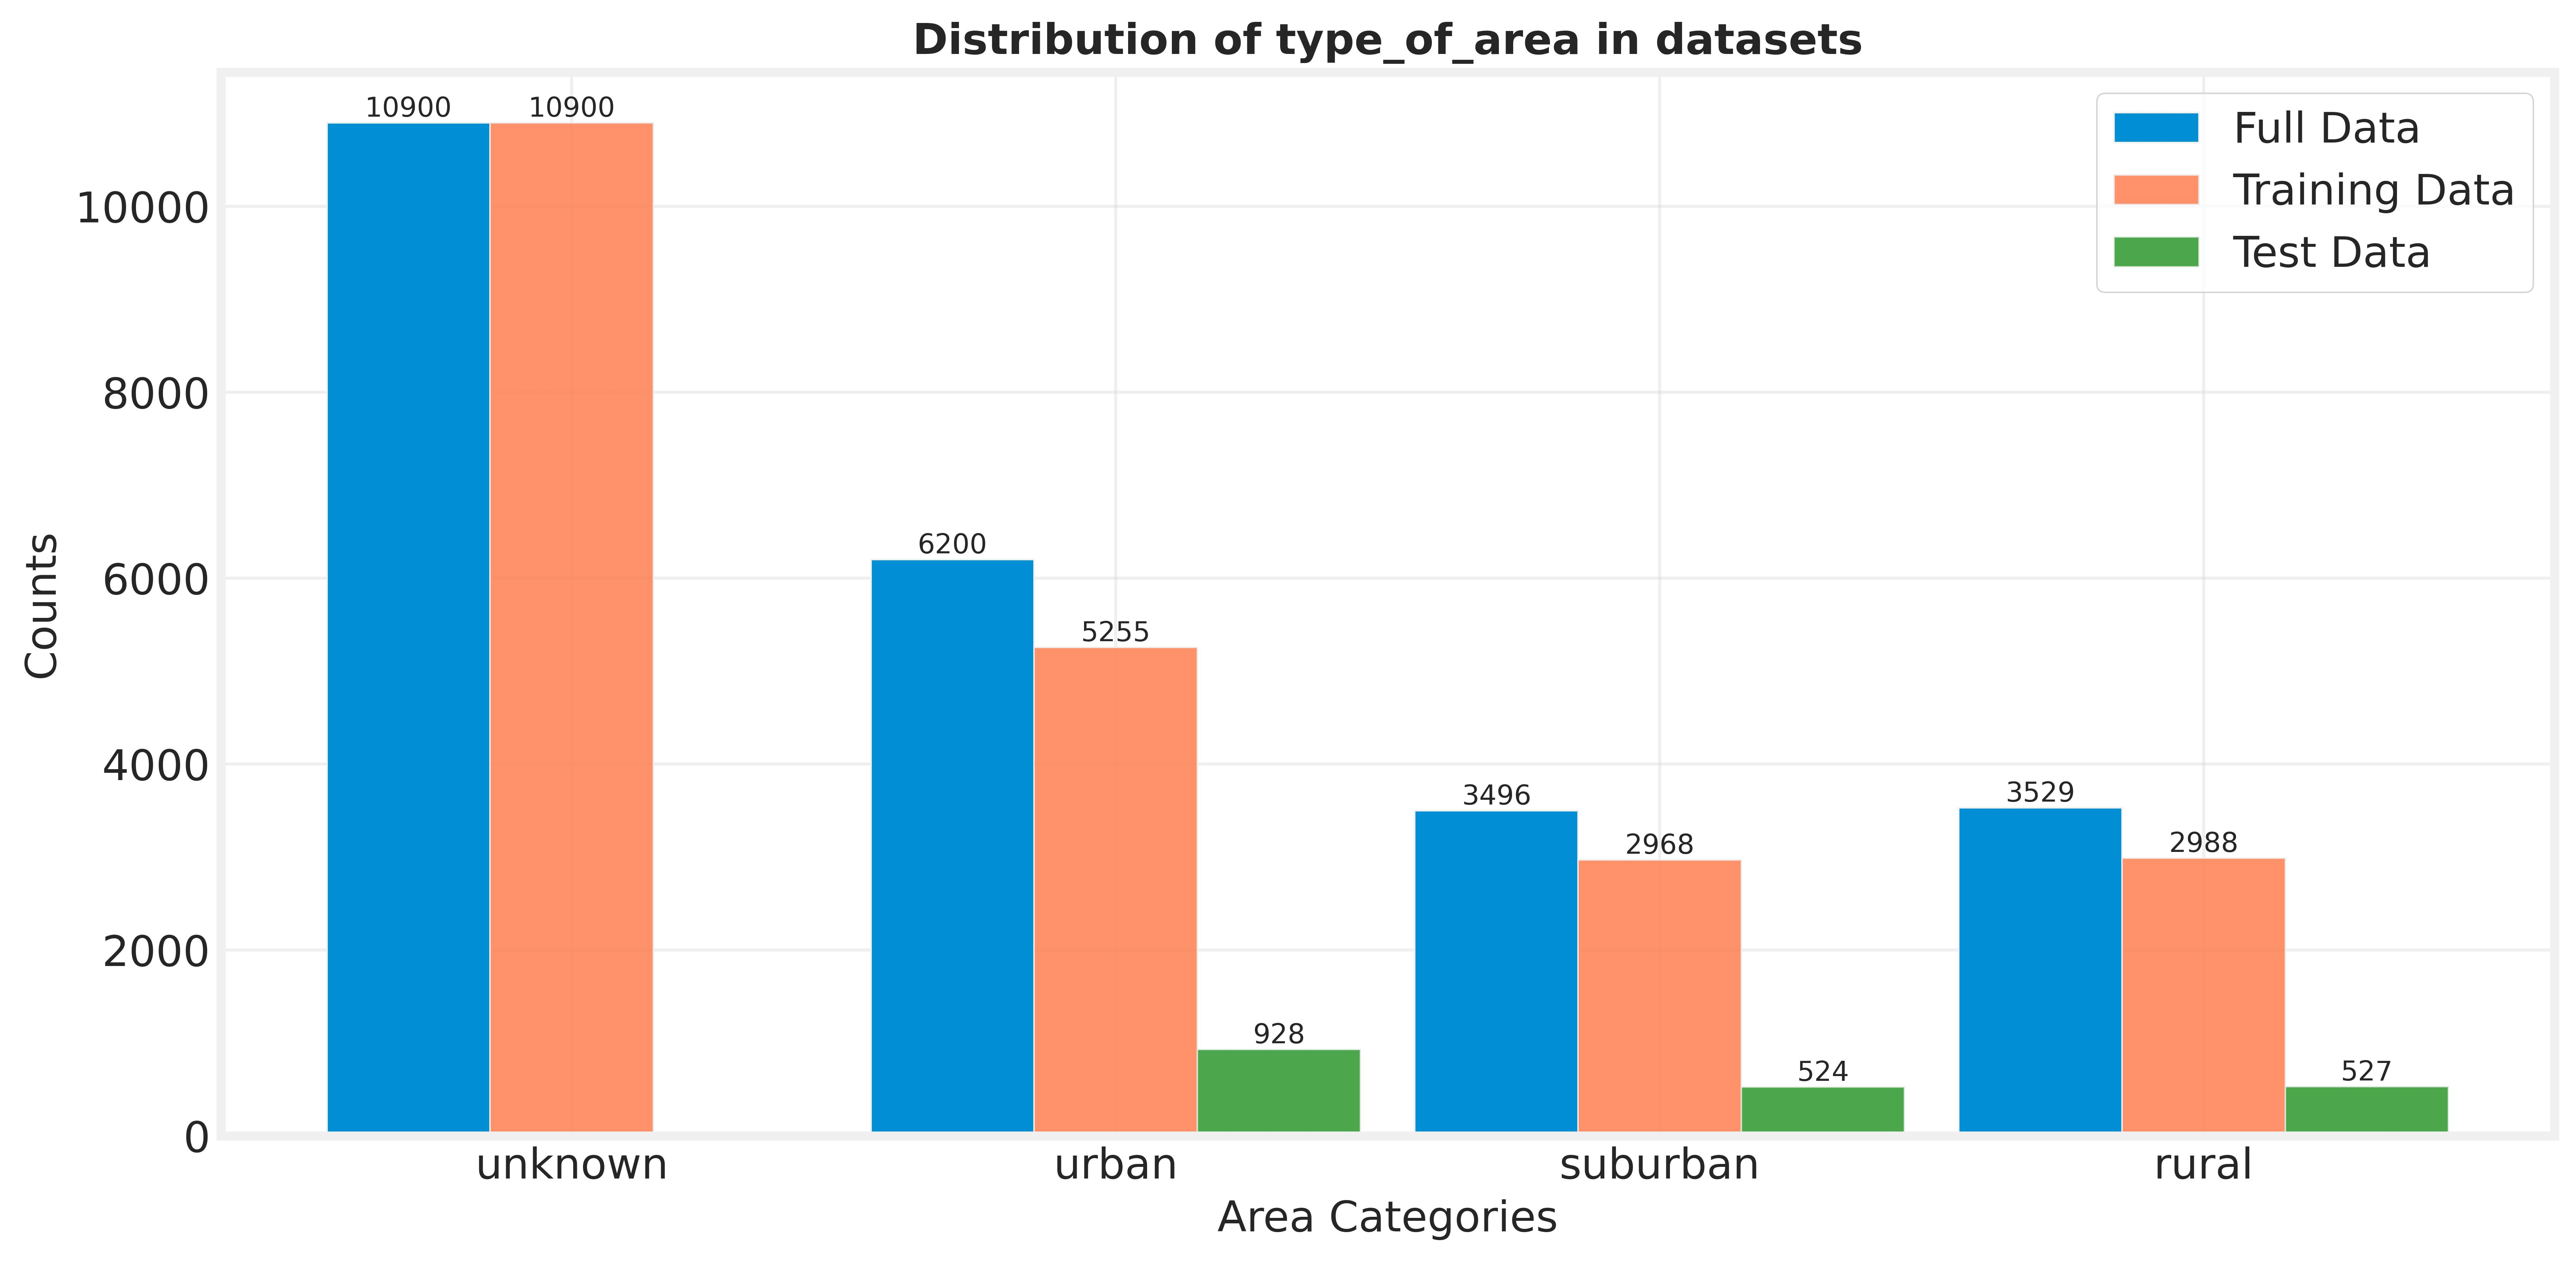
\includegraphics[width=\textwidth,keepaspectratio=true]{figures/data_dist.jpg}
    \caption{Distribution of unlabeled, training, and test data used for the supervised ML models as described in the text}
    \label{data_dist}
\end{figure}

% \begin{figure}[htb!]
%     \centering
%     \subfigure[]{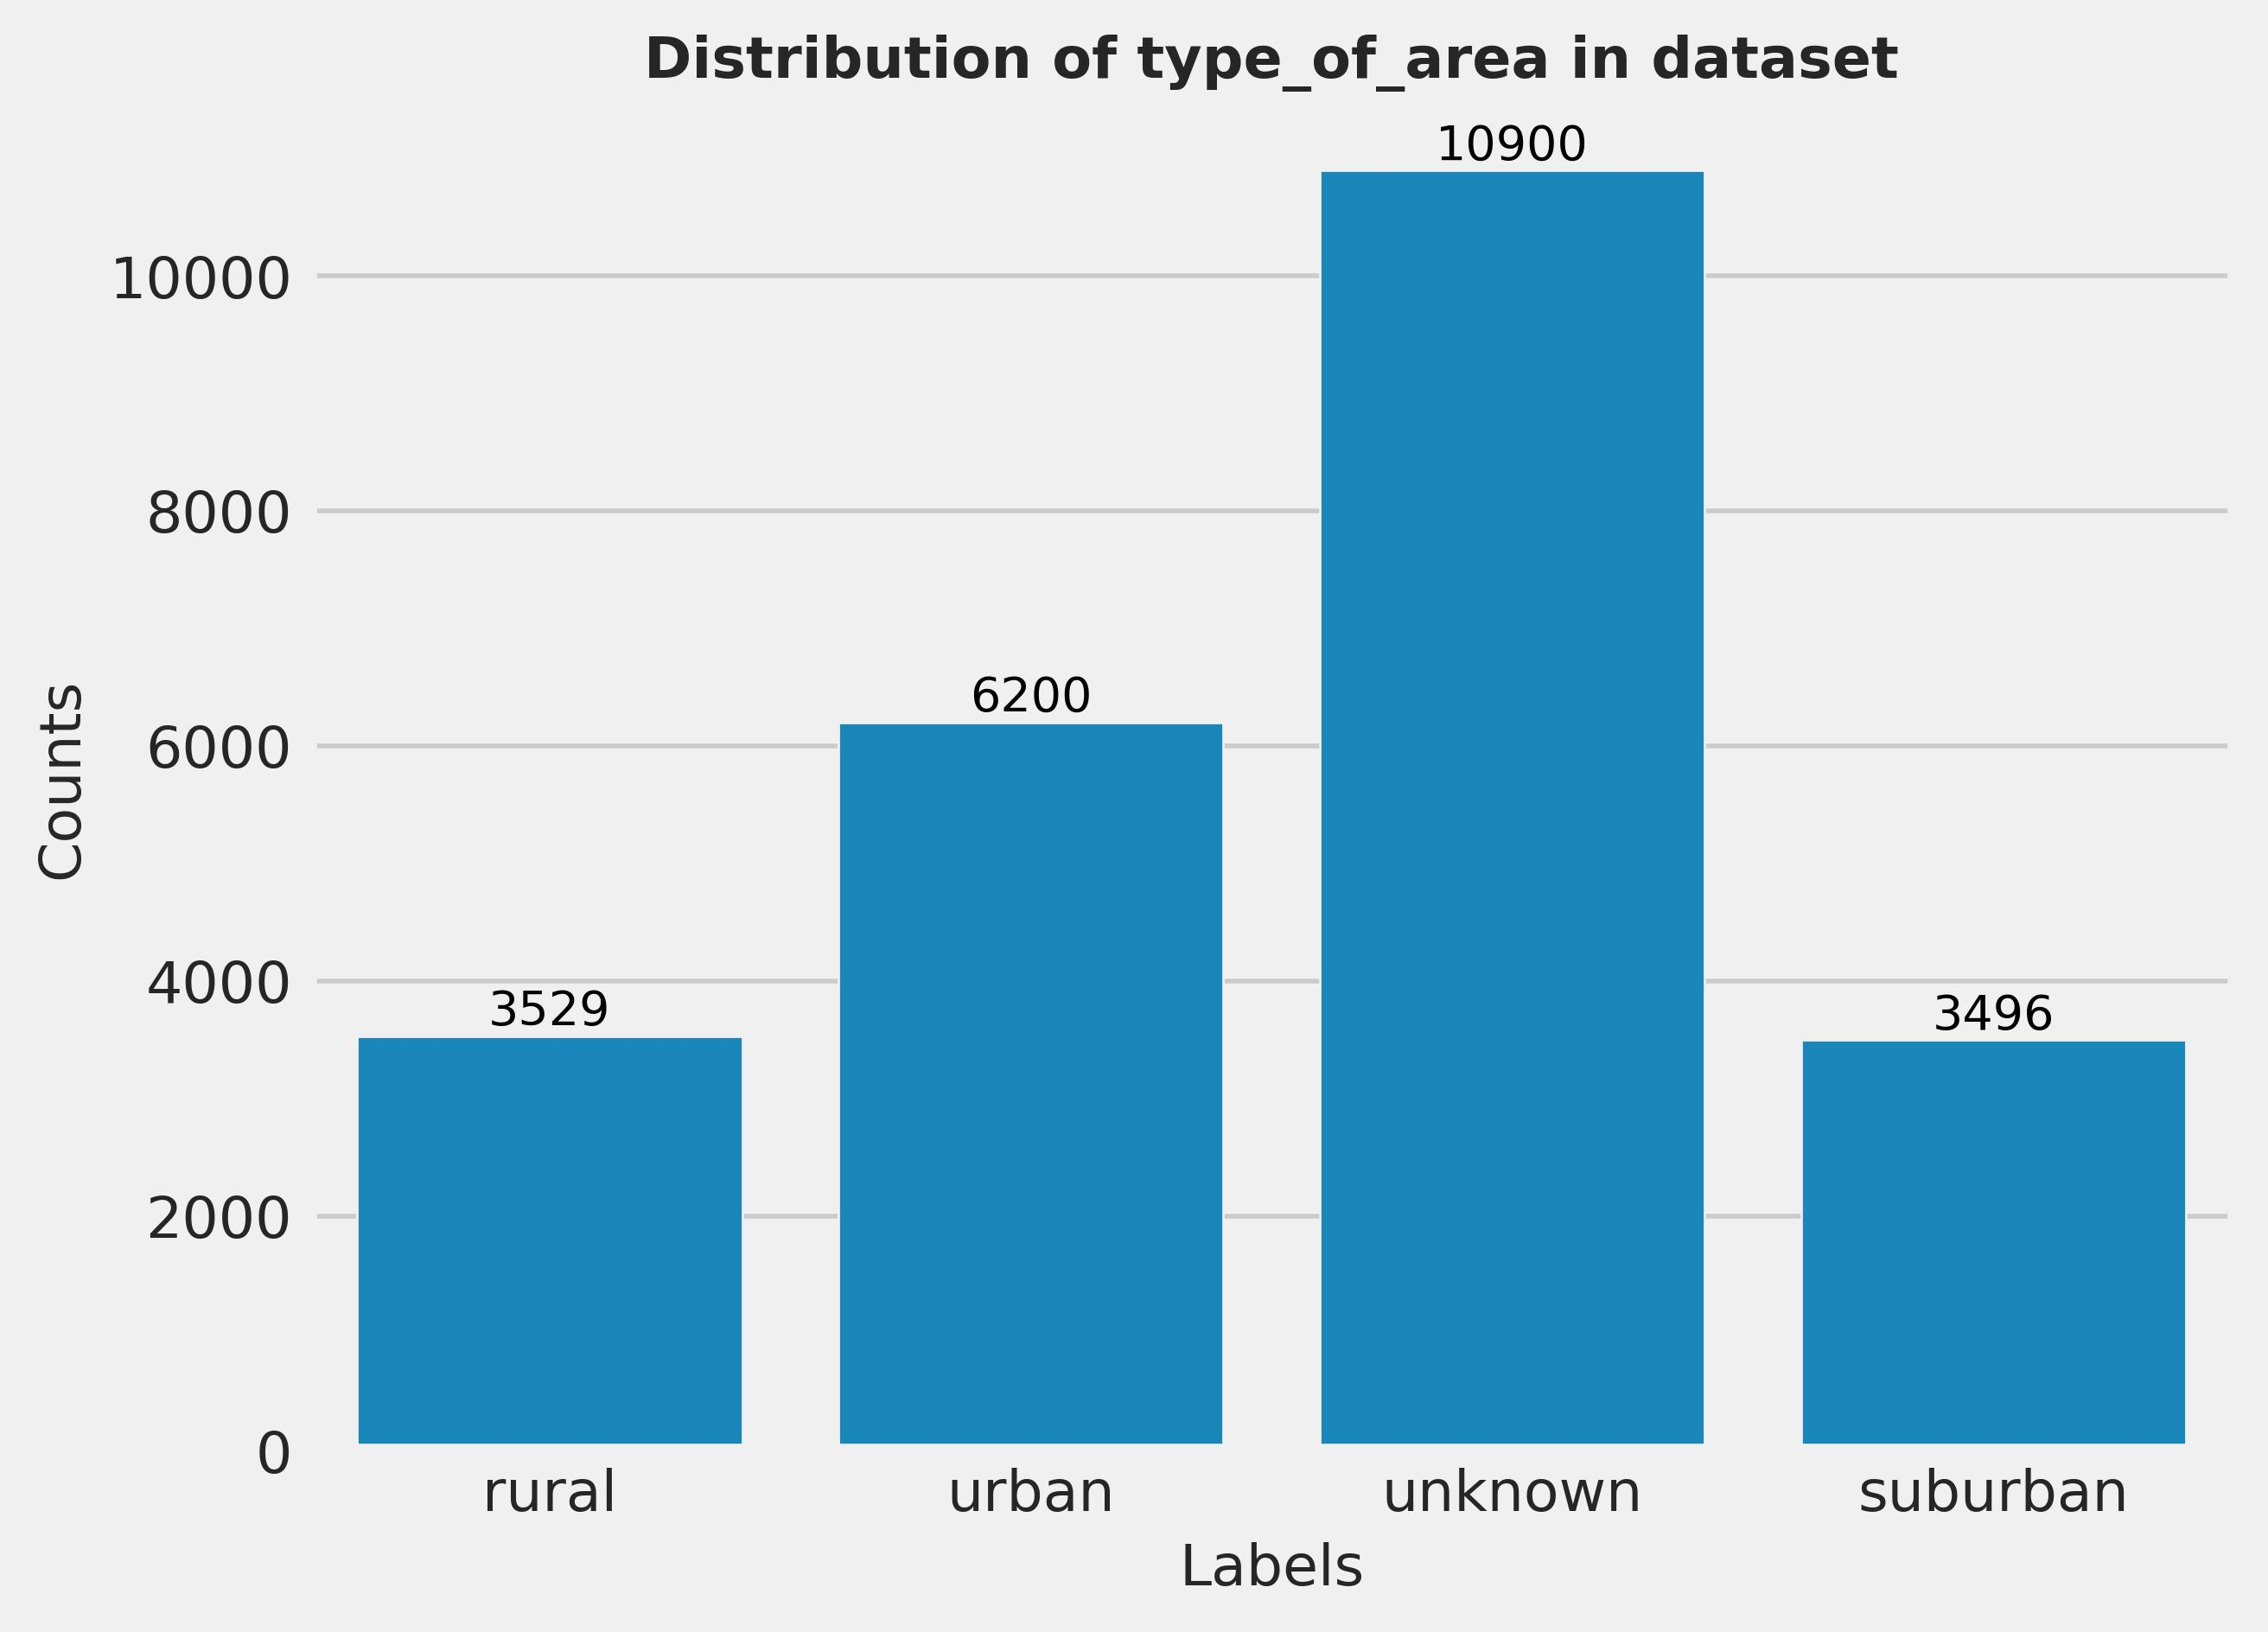
\includegraphics[width=0.49\textwidth]{figures/value_counts_data_type_of_area.jpg} \label{data_dist_a}} 
%     \hskip 0.3cm
%     \subfigure[]{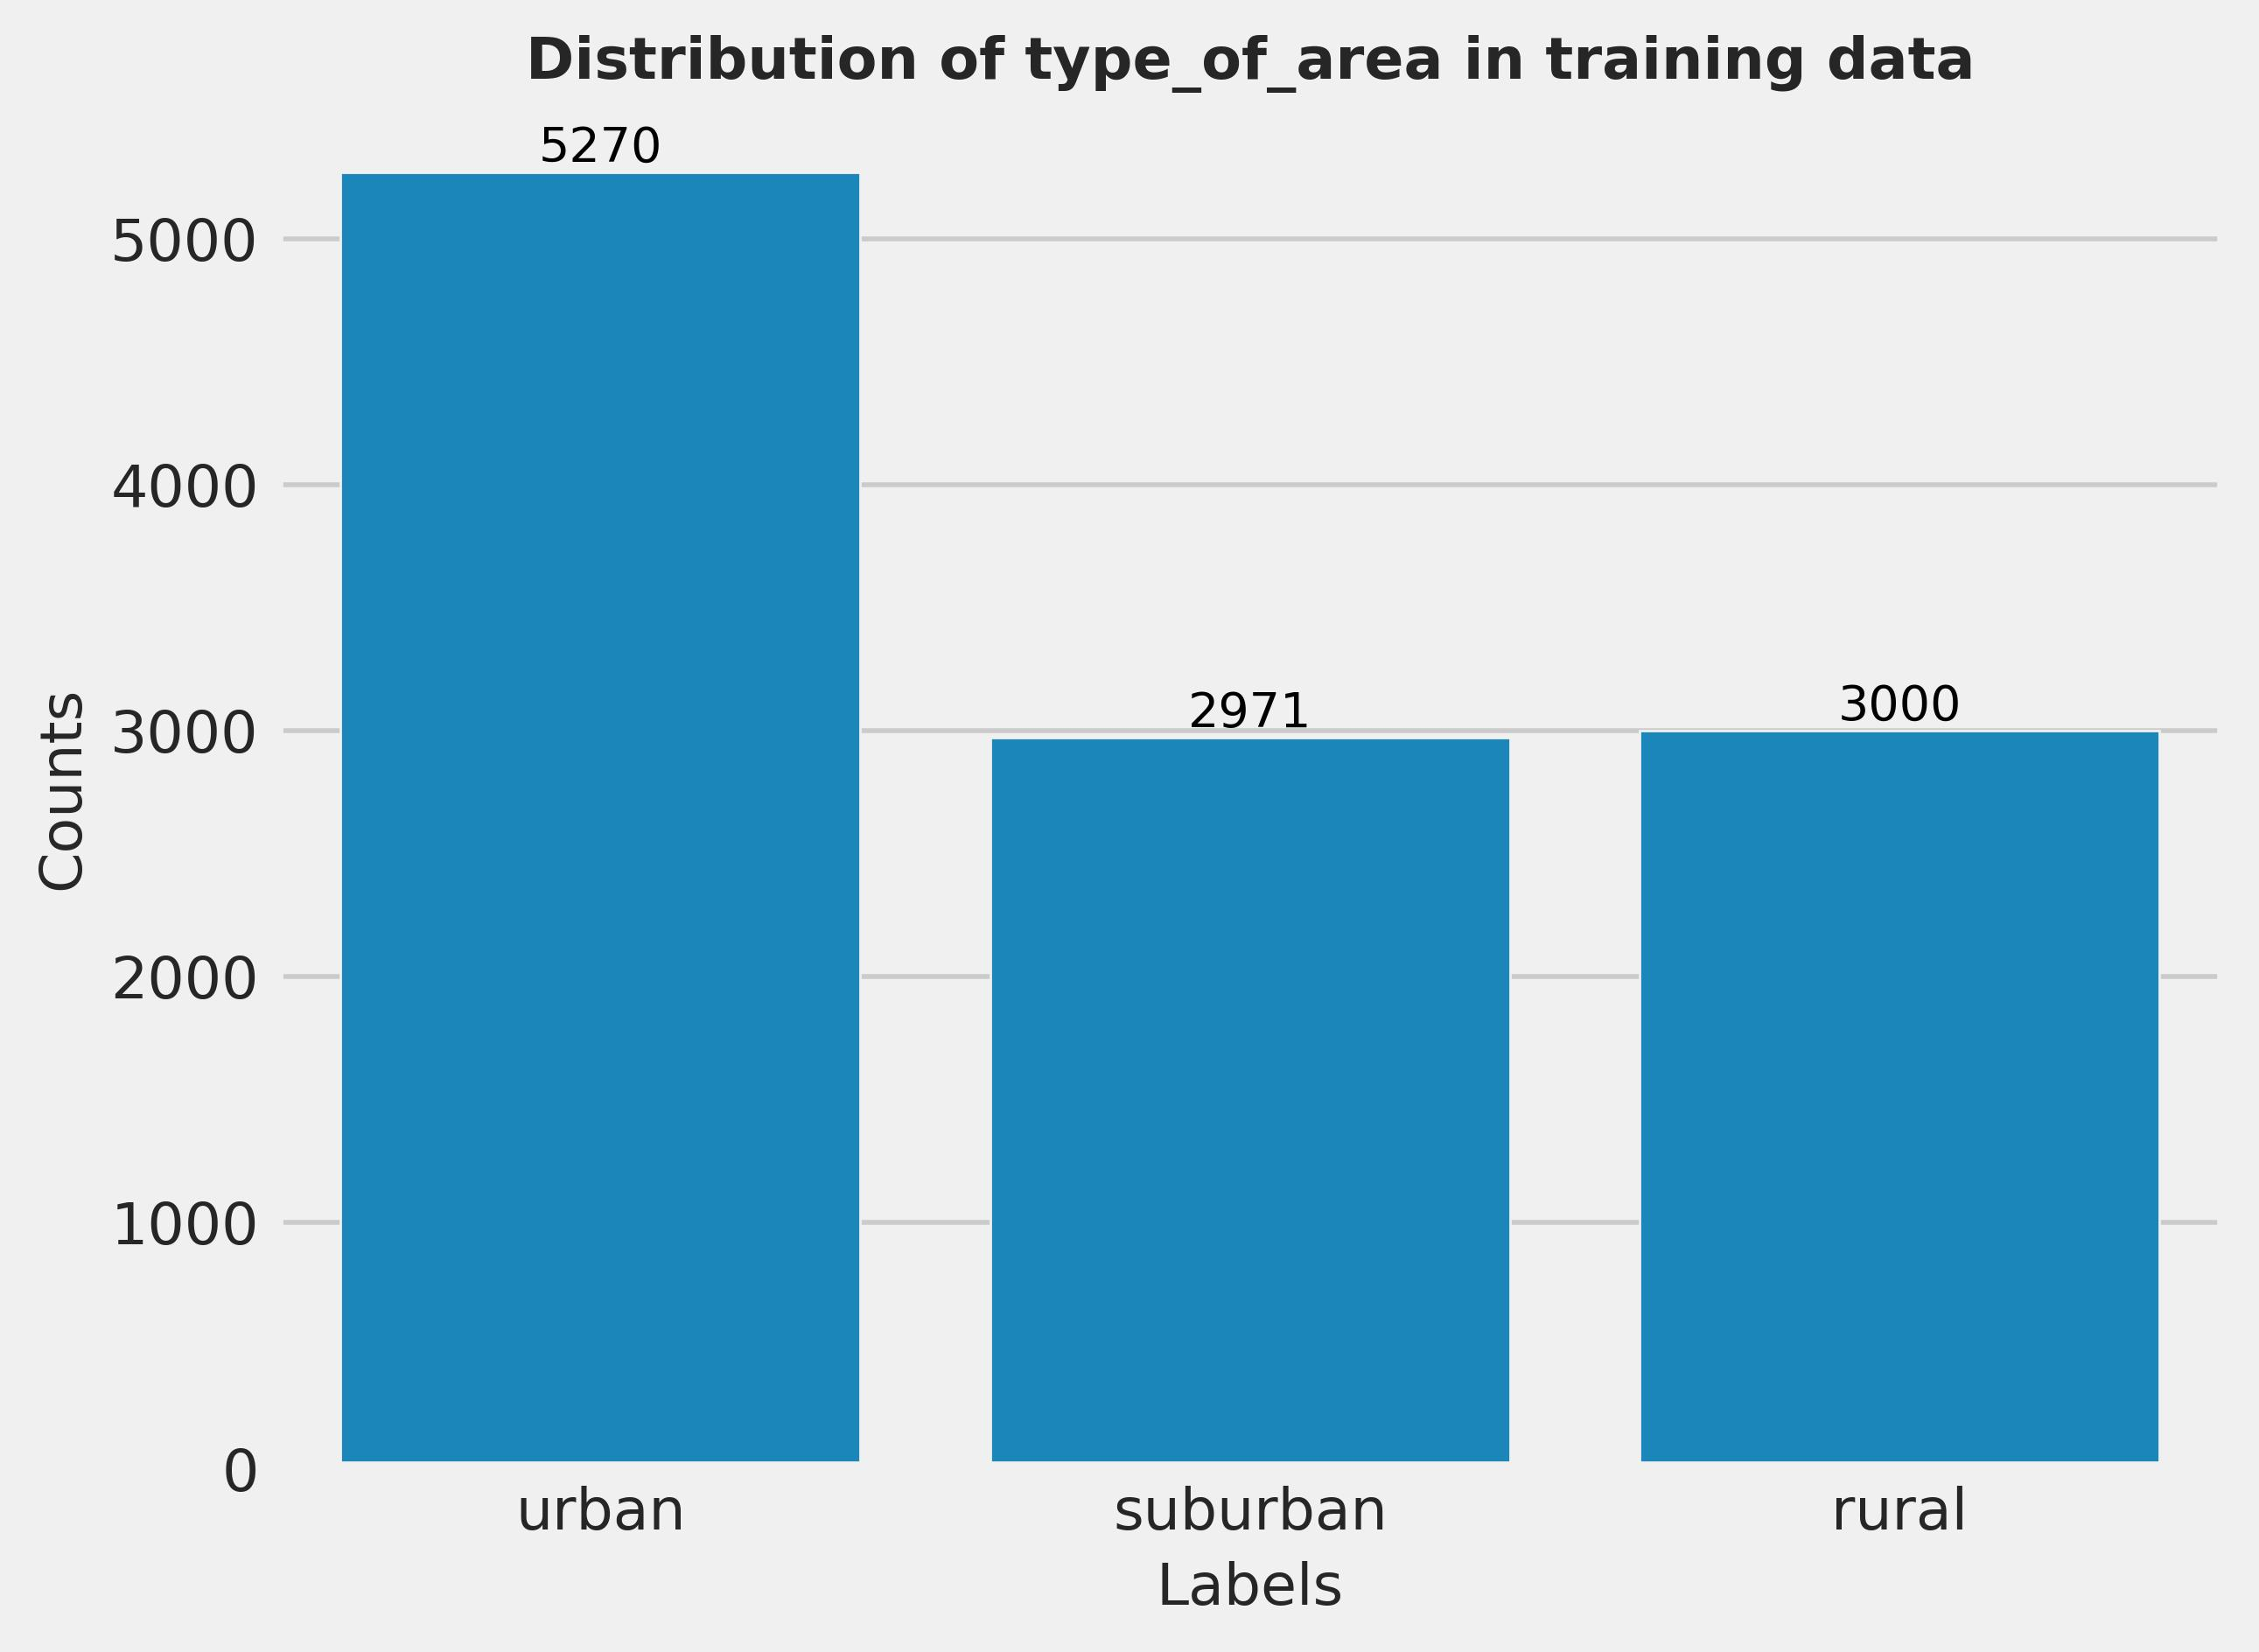
\includegraphics[width=0.48\textwidth]{figures/value_counts_training_data_type_of_area.jpg} \label{data_dist_b}}
%     \caption{(a) Distribution of the entire dataset. (b) Distribution of training data use in supervised learning algorithms.}
% \end{figure}

% \begin{figure}[htb!]
%     \centering
% 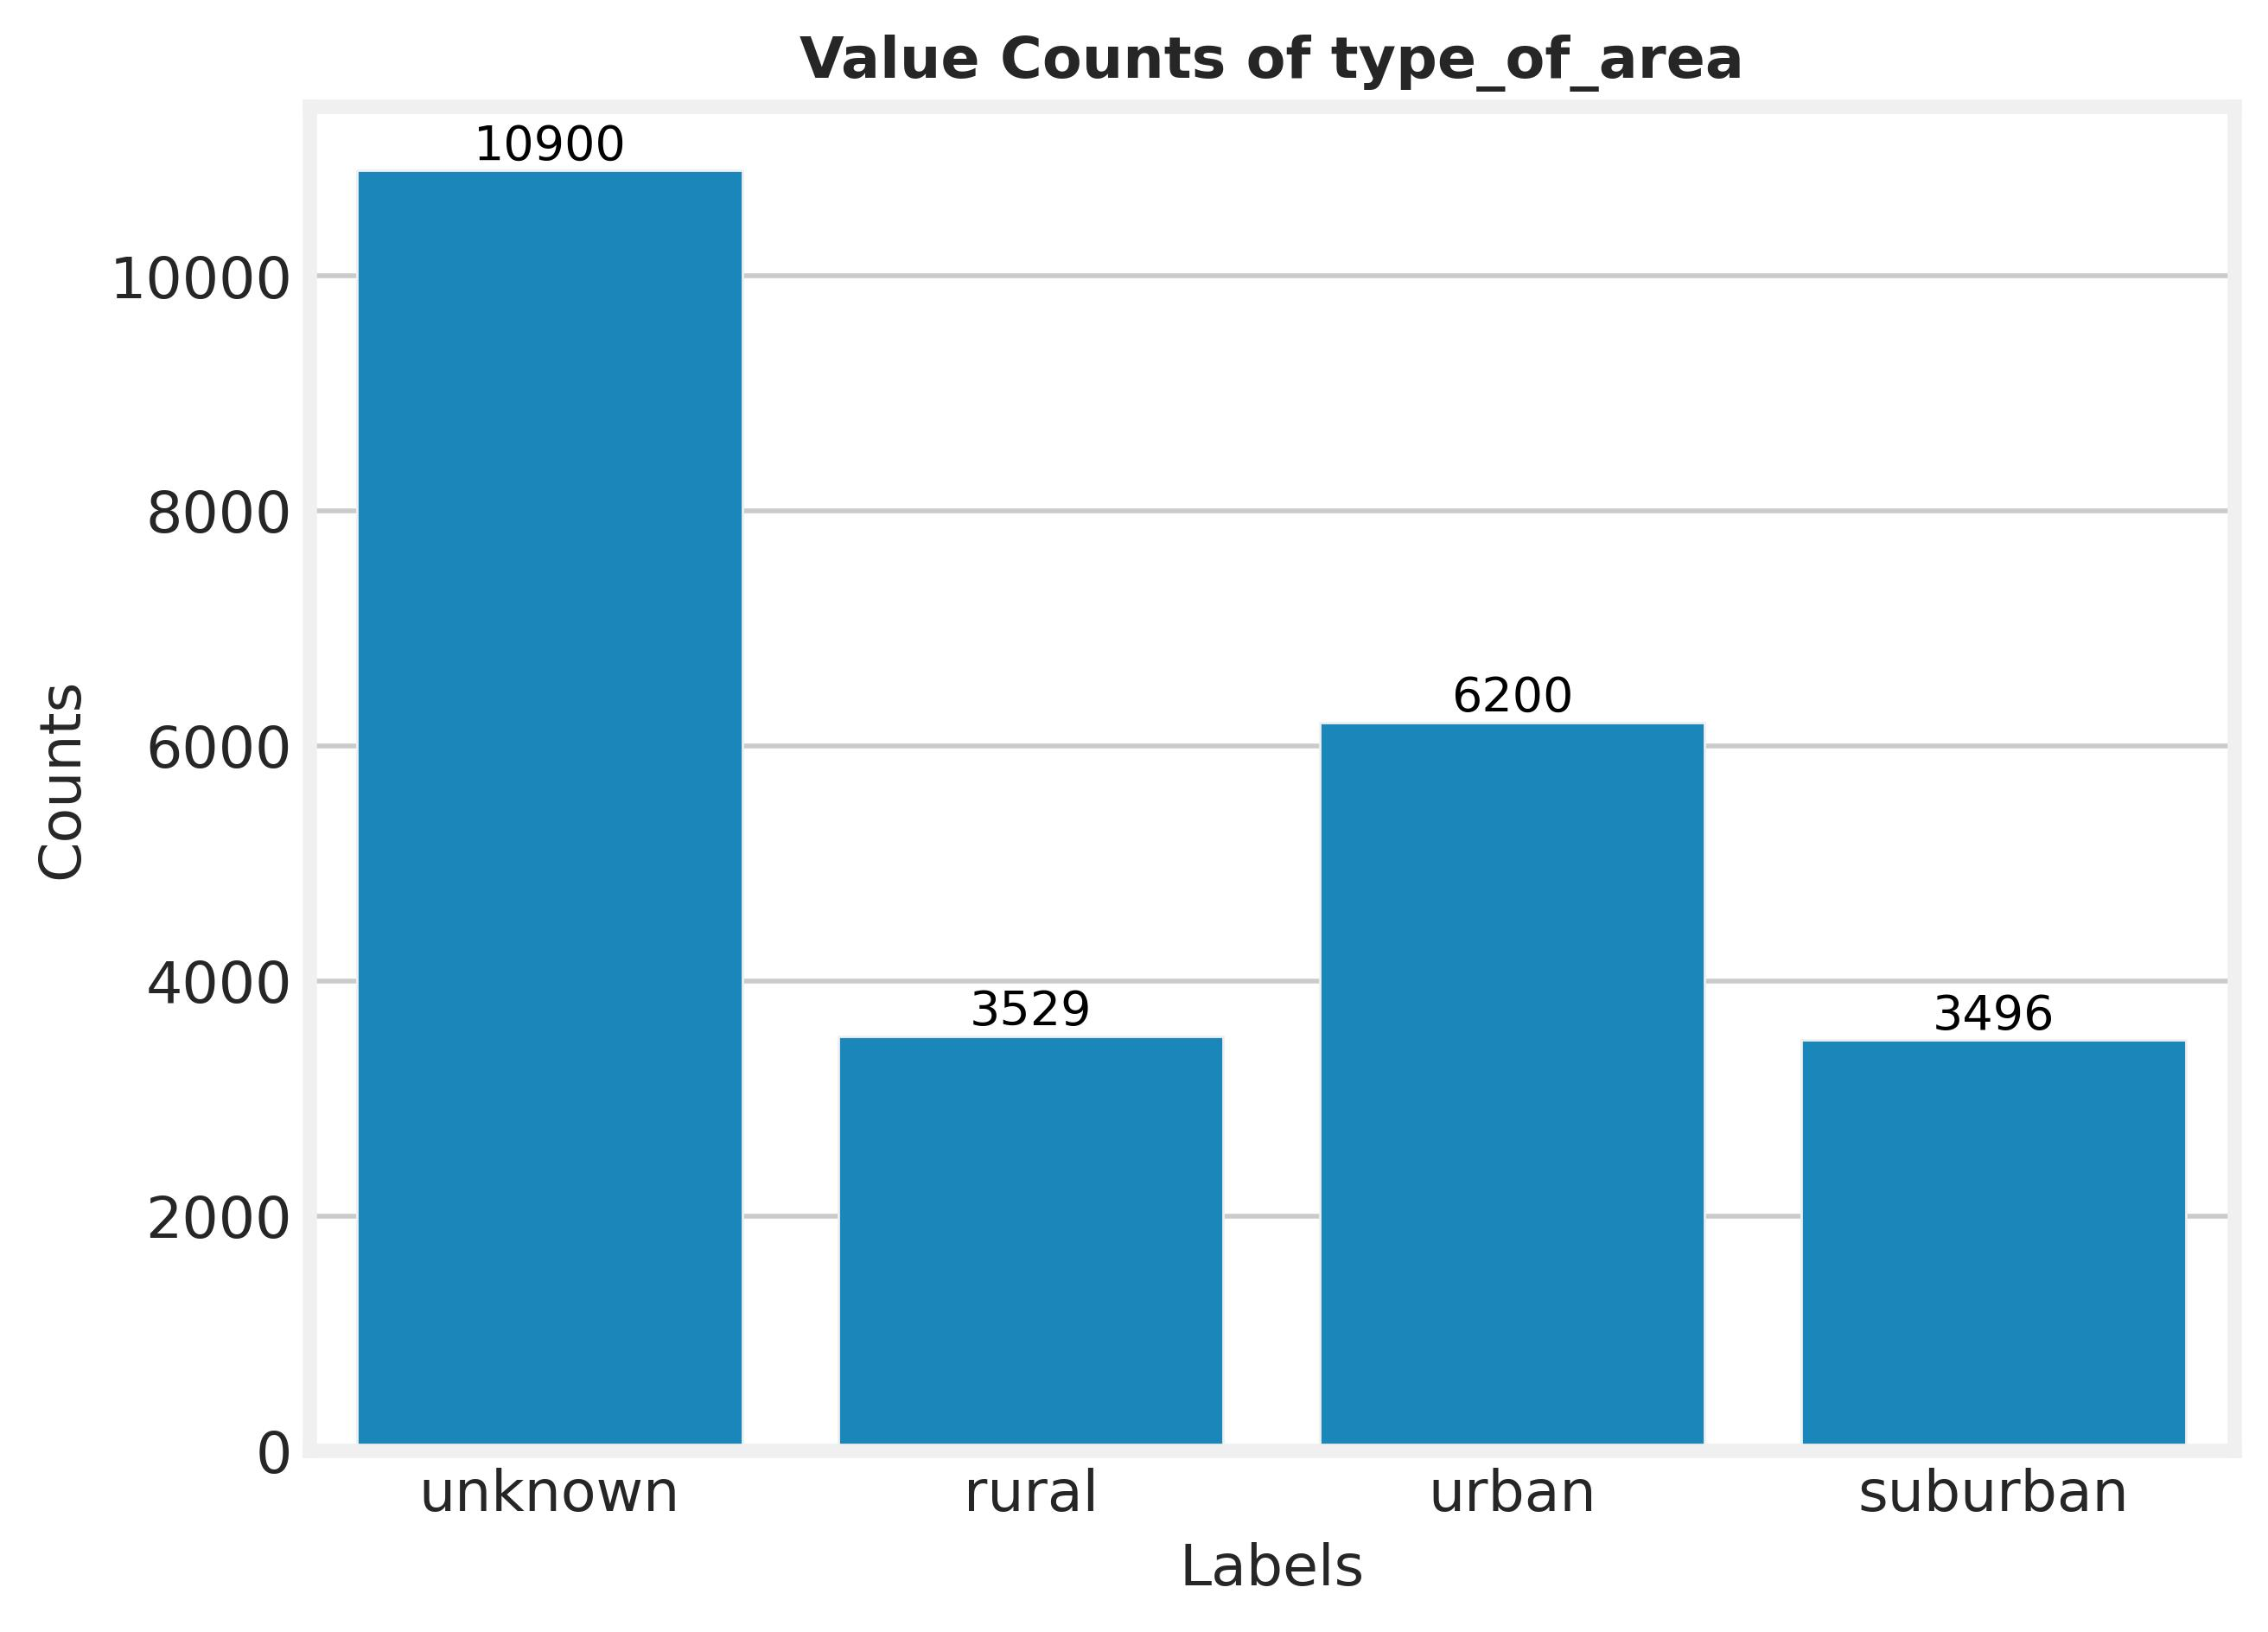
\includegraphics[width=0.65\textwidth,keepaspectratio=true]{figures/value_counts_type_of_area.jpg}
%     \caption{Distribution of different labels in TOAR dataset.}
%     \label{data_dist_a}
% \end{figure}

To ensure the reliability of our machine learning approach, we manually selected 35  stations with clear decision boundaries--that is, stations that are easy to classify as urban, suburban or rural, and excluded them from the training dataset. These stations were explicitly reported by data providers as urban, suburban, or rural, and we used Google Maps \citep{mehta2019google} to manually verify and label them. During this process, we observed discrepancies between the labels provided by the data providers and those derived from our manual Google Maps analysis. Our models will first be evaluated on these 35 stations, with accuracy calculated both against the labels reported by the data providers and against the manually verified labels from Google Maps (referred to as hand-labeled data).

\begin{figure}[htb!]
    \centering
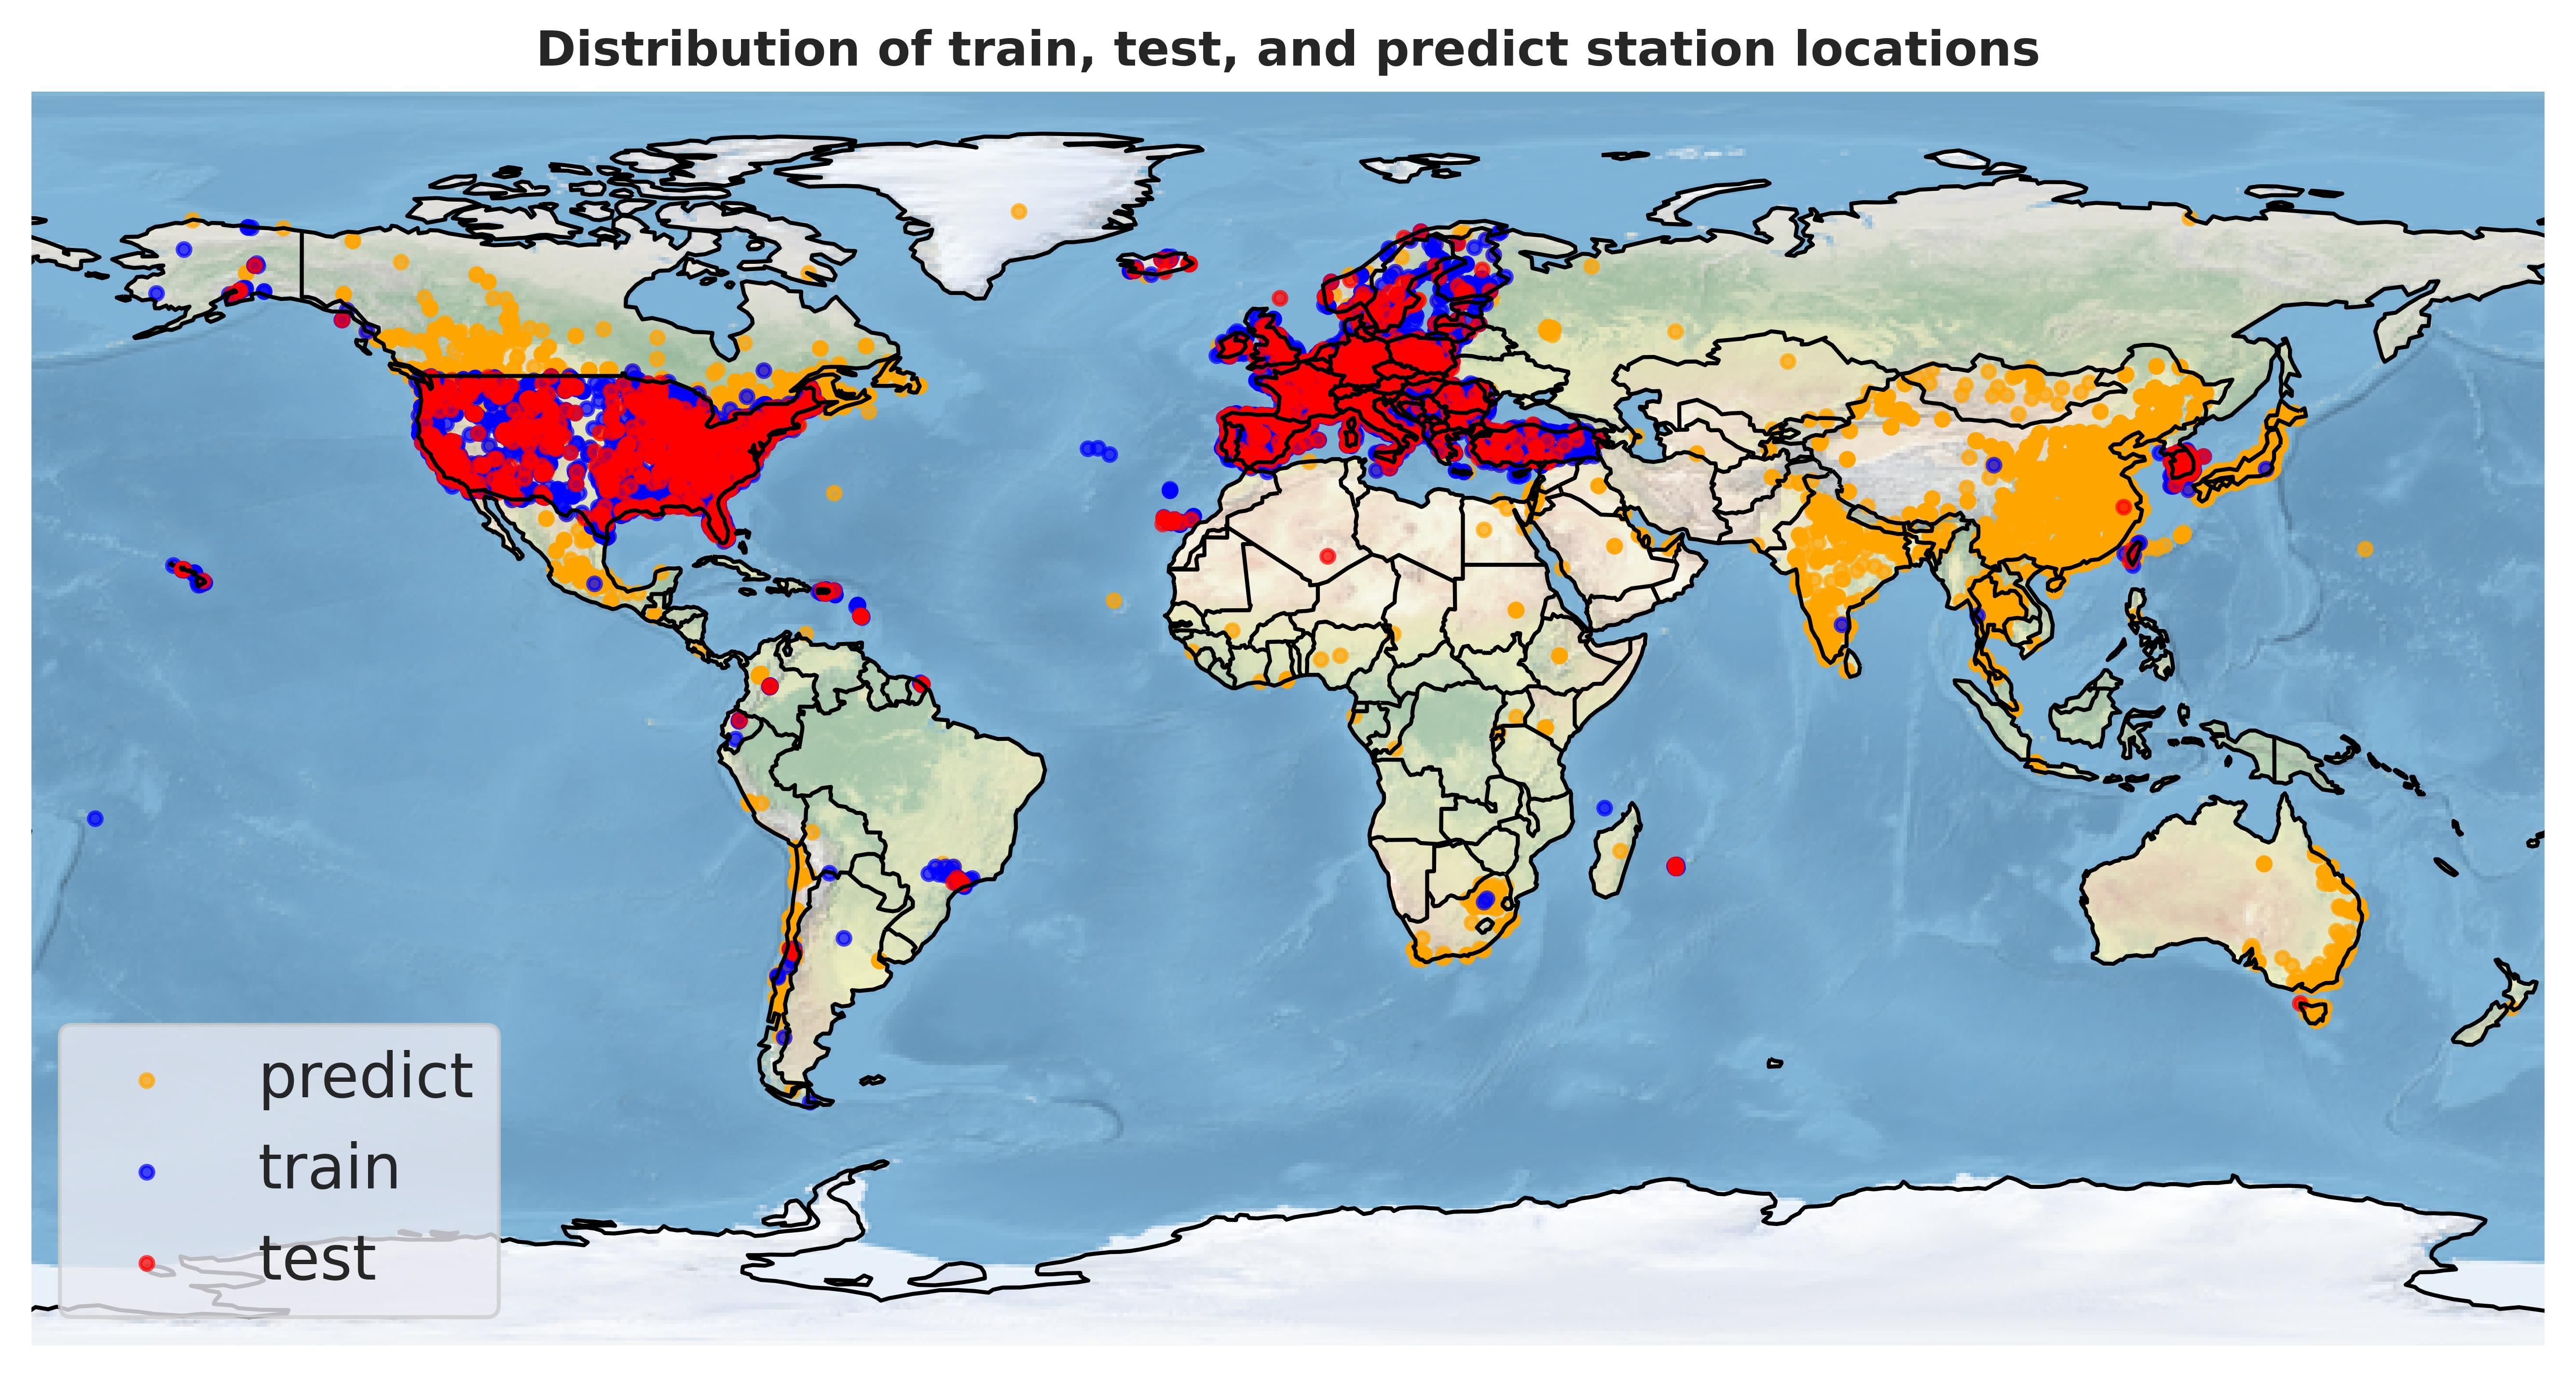
\includegraphics[width=\textwidth,keepaspectratio=true]{figures/data_split.jpg}
    \caption{Distribution of unlabeled, training, and test data used for the supervised ML models as described in the text}
    \label{data_split}
\end{figure}
%\textcolor{B}{Figure 1: It looks as if you primarily predict stations outside the U.S. and Europe. Are the orange dots the 1,000 stations used for testing? Or are these the 9,970 stations lacking classification?} \textcolor{red}{clarify!}

%\textcolor{green}{Figures: I suggest removing the grey background. Check with journal guidelines, but I believe (a) and (b) should be shown above the plot (beside the plot title, if the journal allows the latter).}
%\newpage
\subsection{Machine learning algorithms and evaluation methods}
%\textcolor{B}{Figures 2 and 3: Please introduce PCA as a method to visualize results in the Methods section.} \textcolor{red}{Done!}
This section is devoted to a concise overview of the machine learning techniques employed in this study. Additionally, we describe the evaluation metrics used to quantify the effectiveness and accuracy of our models.
%This section briefly overviews the machine learning techniques employed in this study. These include the unsupervised learning method, K-means, and supervised classifiers such as random forest, lightGBM, and CatBoost algorithms. Additionally, we present the evaluation metrics utilized to gauge the effectiveness and accuracy of our machine learning models.
% remove this subsubsection and instead "elevate" the \texbf labels to subsubsections?
\subsubsection{Machine learning algorithms}
\begin{itemize}
    \item \textbf{K-means clustering} is a widely-used unsupervised machine learning technique that aims to partition data into k distinct groups called clusters \cite{bahmani2012scalable, sinaga2020unsupervised, pelleg2000x}. Each data point is assigned to the cluster with the nearest centroid. The algorithm seeks to minimize the within-cluster sum of squares, which measures the squared distances between data points and their respective centroids. % mean, also known as the cluster is a popular unsupervised machine learning model that aims to partition data into $k$ groups called clusters, in which each data point belongs to the cluster with the nearest mean(cluster centroid) \cite{sinaga2020unsupervised}. 
    %% I find this description somewhat convoluted and imprecise. Where do the mean values come from? I think it is important to mention the iterative procedure and state that mean values are calculated so that the overall distance metric is minimized. Out of curiosity (we discussed this a bit in Olga Lyapina's paper): would it make sense to (also) try to maximize the separation between clusters? Or is this mathematically the same thing?
    %K-means seeks to minimize the within-cluster sum of squares, which measures the squared distances between data points and their respective centroids.
    One key requirement of K-means is specifying the number of clusters beforehand. We employed the heuristic elbow method to determine the appropriate number of clusters for our task. The elbow method is a heuristic technique used to determine the optimal number of clusters in K-means clustering. It works by plotting the within-cluster sum of squares (WCSS) as a function of the number of clusters and identifying the "elbow" point on the curve, which correspond to the optimal number of clusters \citep{ketchen1996application}.
    %as illustrated in Figure~\ref{data_split}.
    %In the K-means algorithm, it is necessary to specify the number of clusters beforehand. We use the heuristic elbow method to determine the number of clusters that would be appropriate for this task, see Figure~\ref{elbow}. 
    In our K-means clustering application, we determine that three clusters are optimal (see Figure~\ref{elbow}), which aligns well with our objective of categorizing the stations into three groups: urban, suburban, and rural. 
    However, it is important to note that visual inspection of correlation plots between individual metadata values Figure~\ref{data_split} reveals rather fuzzy boundaries between clusters. This observation aligns with our expectations, given the diverse nature of urban, suburban, and rural locations across different countries, which can vary significantly in terms of industrial development, population density, and degree of urbanization in different countries \citep{zhang2024promoting}.
    %We note, however, that visual inspection of correlation plots between individual metadata values indicates a rather fuzzy boundary between clusters. This coincides with our expectation as there are very different types of urban, suburban, and rural locations depending on the industrial development, population density, and degree of urbanization in different countries.
    \item  \textbf{Random Forest classifier}  is a widely-used machine learning algorithm for classification tasks. As an ensemble learning method, it constructs multiple decision trees through bagging during training and outputs the class that is predicted by the majority vote of the individual trees \citep{breiman2001random}. Known for its robustness, it naturally resists overfitting through random feature selection and typically requires minimal tuning compared to other algorithms.
    In our implementation, we train the Random Forest classifier with 500 estimators, employing entropy as the optimization criterion. These specific hyperparameters were determined through a grid search. We utilize the RandomForestClassifier from the scikit-learn library \citep{scikit-learn}.
    
    \item  \textbf{The LightGBM (LGBM) classifier} is a supervised machine learning algorithm that utilizes gradient boosting techniques and tree-based learning. It employs histogram-based algorithms and leaf-wise tree growth strategies, which contribute to accelerated training speeds and reduced memory consumption. 
    %It's designed to be highly efficient, offering fast training speeds, low memory usage, and excellent performance. 
    LightGBM is particularly well-suited for handling large-scale datasets. Its lightweight architecture and optimized algorithm make it a popular choice for tasks requiring both speed and accuracy in prediction \citep{ke2017lightgbm}.  In our implementation, we train LightGBM with 500 estimators using Python's open-source library 'lightgbm' \citep{van2007python}.
%% [mgs] This description raises the question of why we use it. We don't have a very large dataset that must be trained on a distributed system. Are there other = quality advantages??    
 %   In our implementation, the default hyperparameters yield better accuracy. 
%% [mgs] better compared to what??
   % LGBM is available as an open-source Python library.
    \item  \textbf{The CatBoost classifier}  is a machine learning algorithm that uses gradient boosting on decision trees, specifically designed to handle categorical features seamlessly \cite{prokhorenkova2018catboost}. CatBoost stands for "Categorical Boosting" and automatically handles categorical variables  without requiring manual prepossessing. It uses symmetric trees and ordered boosting to prevent overfitting, and often outperforms other methods on datasets with categorical data.
    This  makes it an attractive option for datasets containing both numerical and categorical variables. In our implementation, we employ the open-source CatBoost library and configure the model with 500 estimators to balance performance and computational efficiency.
\item \textbf{The Voting Classifier} is an ensemble meta-estimator that combines predictions from multiple base models to enhance overall accuracy and robustness. It functions by either majority vote ('hard') or averaging predicted probabilities ('soft'), effectively balancing the weaknesses of individual classifiers. This approach often yields superior generalization and reduced overfitting. Our implementation uses a soft voting strategy to aggregate predictions from a Random Forest, LightGBM, and CatBoost classifier via the scikit-learn library. \citep{scikit-learn}
\end{itemize}

\subsubsection{Leveraging Model Uncertainty to Enhance Suburban Classification Accuracy}
Considering the inherent subjectivity in defining suburban areas, we refined our prediction methodology as follows: For any given station, if the model's highest probability for either urban or rural classification falls below a threshold, and if the second-highest probability corresponds to suburban classification, we interpret this as the model's uncertainty in categorizing the area between rural and suburban, or urban and suburban. In such cases, we classify the station as suburban. We applied the grid-search strategy in the range [0.35, 0.85] minimizing macro-F1, to find optimal threshold for each supervised algorithms. We obtain the thresholds of 0.5214, 0.4357, 0.5459, 0.4846 for random forest, CatBoost, LightGBM, and voting respectively. This approach acknowledges the model's indecision and leverages it to better capture the nuanced nature of suburban environments.
\subsubsection{Evaluation}
To evaluate our model's accuracy, we use a separate test dataset of 1,979 samples, shown as red dots in Figure~\ref{data_split}. The test dataset consists of samples that were selected with stratification to ensure it reflects the distribution of real data, and intentionally excluded from both the training phase and the hyperparameter tuning process. This approach ensures that the evaluation metrics provide an unbiased assessment of the model's ability to generalize to new, unseen data, challenging the model in the real-world application scenario. We employed the following evaluation metrics to measure the performance of our machine learning model on this test dataset.

\begin{itemize}
\item  \textbf{Accuracy} measures the ability of the machine learning model to accurately predict the outcome for the given input data. It is measured as the proportion of correct predictions to the total number of predictions made by the model, and given by the following formula:
$$\mathrm{Accuracy} = \frac{\#\mathrm{Correct ~Predictions}}{\# \mathrm{Total~ Predictions}
}\times 100$$
Here and in the following formulas, \# stands for "Number of"
\item \textbf{Per-class Precision:} For a given class $c$, precision quantifies the fraction of correctly predicted instances of class $c$ among all instances that the model predicted as class $c$:
$$
\mathrm{Precision(c)} = \frac{\#\mathrm{True~Positives}(c)}{\#\mathrm{True~Positives}(c) + \#\mathrm{False~Positives}(c)}\times 100$$
    Here, True Positives (TP) are the instances that actually belong to class $c$ and were correctly predicted as such, while False Positives (FP) are the instances that do not belong to class $c$ but were incorrectly predicted as instance of class $c$. Precision reflects how reliable predictions of class $c$ are: high precision indicates that when the model predicts $c$, it is usually correct \citep{powers2020evaluation, brodersen2010balanced}.
\item \textbf{Per-class Recall (Sensitivity, True Positive Rate):}  
For a given class $c$, recall is defined as the proportion of true positive predictions for class $c$ among all actual instances belonging to class $c$
$$
\mathrm{Recall}(c) = \frac{\#\mathrm{True~Positives}(c)}{\#\mathrm{True~Positives}(c)~ + ~\#\mathrm{False~Negatives}(c)} \times 100$$ Here, False Negatives are the instances of class $c$ that the model incorrectly assigned to another class. 
Recall characterizes the ability of the model to retrieve all relevant instances of class $c$; high recall indicates that the model rarely overlooks samples from this class \citep{powers2020evaluation}.

\item \textbf{Per-class F1 Score:} The F1 score for class $c$ is defined as the harmonic mean of precision and recall:
$$\mathrm{F1}(c) = \frac{2\cdot \mathrm{Precision}(c)\cdot \mathrm{Recall}(c)}{\mathrm{Precision}(c)~ + ~ \mathrm{Recall}(c)} \times 100$$
This metric provides a single, balanced measure of a model's ability to achieve both high precision and high recall for class $c$, penalizing extreme values in either criterion. A high F1 score indicates that the classifier is effective both in accurately identifying instances of class $c$ as well as capturing the majority of actual class $c$ samples \citep{powers2020evaluation}.
 (recall).
\item \textbf{Macro-F1:} The macro-averaged F1 score is computed as the arithmetic mean of the per-class F1 scores, assigning equal weight to each class irrespective of its prevalence in the dataset:
$$\mathrm{Macro\text{-}F1} = \frac{1}{N} \sum_{c=1}^{N} \mathrm{F1}(c) \times 100$$
%$$Macro-F1 = \frac{1}{N}\sum_{c=1}^{N}F1(c)$$
where $N$ denotes the total number of classes. This metric evaluates overall model performance by averaging across all classes and penalizes poor classification performance on minority classes, as each class contributes equally to the final score \citep{powers2020evaluation}. Macro-F1 is widely used in multi-class classification evaluation for its insensitivity to class imbalance \citep{brodersen2010balanced}.
\item \textbf{Balanced Accuracy:} Balanced accuracy is defined as the average of the per-class recall values:
$$\mathrm{Balanced\ Accuracy} = \frac{1}{N} \sum_{c=1}^{N} \mathrm{Recall}(c) \times 100 $$
where $N$ represents the total number of classes. Unlike standard accuracy, balanced accuracy accounts for class imbalance by assigning equal weight to each class regardless of sample frequency. This metric provides a more equitable evaluation in imbalanced classification scenarios, mitigating the bias introduced when a dominant class disproportionately influences the overall accuracy score \cite{brodersen2010balanced, sensoressa2024balanced}.
% \item \textbf{Balanced Accuracy: } Average of per-class recalls.
% $$Balanced~ Accuracy =  \frac{1}{N}\sum_{c=1}^{N}Recall(c)$$
% It is fair version of accuracy that handles imbalanced datasets by giving each class equal importance. Standard accuracy can be misleading if one class dominates; balanced accuracy avoids this by normalizing per class.


 \item  \textbf{Adjusted Rand Index(ARI)}  quantifies the similarity between the true cluster assignments and those predicted by the model. It operates by considering all possible pairs of samples and counting how many pairs are assigned to the same or different clusters in both the predicted and true clusters, \cite{chacon2023minimum, chekir20173d}. The ARI score ranges from -1.0 to 1.0. A score approaching 1 indicates strong concordance between the true labels and the model's predictions, indicating that many sample pairs are clustered similarly in both clusters. A score near 0 suggests the clustering is comparable to random assignment. A negative score suggests that the predicted clusters frequently disagree with the true clusters, potentially performing worse than random assignment. This implies that sample pairs are often grouped differently in the predicted clusters compared to the true clusters.
 %A negative score indicates a level of disagreement between the true and predicted clusters, potentially worse than random assignment, implying that sample pairs are often grouped differently in the two clusters.
% {\bf but this doesn't explain what the ARI evaluates. You may want to write down the formula here.}
% The Adjusted Rand Index (ARI) quantifies the similarity between the true cluster assignments and those predicted by the algorithm. It operates by considering all possible pairs of samples and counting how many pairs are assigned to the same or different clusters in both the predicted and true clusters. The ARI score ranges from -1.0 to 1.0. A score approaching 1 signifies strong concordance between the true labels and the algorithm's predictions, indicating that many sample pairs are clustered similarly in both groupings. A score near 0 suggests the clustering is comparable to random assignment. A negative score indicates a level of disagreement between the true and predicted clusters, potentially worse than random assignment, implying that sample pairs are often grouped differently in the two clusters.
\item \textbf{Normalized Mutual Information (NMI)} measures the mutual information between the true clusters of the samples and the clusters assigned by K-means, normalized by the average entropy of the two label sets. It ranges from 0 to 1, where a score close to 1 indicates strong agreement between the true clusters and the K-means clusters. A score of 0 indicates no mutual information between clusters \citep{kvaalseth2017normalized}.
\end{itemize}
To visualize the K-means clusters, we employed Principal Component Analysis (PCA), a dimensionality reduction technique that projects data onto orthogonal axes of maximum variance, enabling the representation of high-dimensional data in two or three dimensions. \citep{abdi2010principal}.
%It is widely used to reveal patterns, clusters, and outliers during exploratory data analysis. In our implementation, we apply PCA using scikit-learn to reduce the data to two components for visualization of K-means cluster, see Figure~\ref{k-means_cluster1}, and Figure~\ref{kmean_cluter2}} \textcolor{blue}{To be removed!}
\section{Results and discussion} \label{results_discusion}
In this section, we present and analyze the results of the various machine learning models applied to the TOAR station classification task. The first subsection details the outcomes of the unsupervised K-means clustering. The second subsection presents and analyzes the results from the three supervised methods. Finally, the last subsection discusses the overall performance and comparative insights of the different approaches.
\subsection{Results for K-means clustering}
Figure~\ref{data_split} shows the elbow plot, a heuristic technique used to determine the optimal number of clusters for K-means clustering. As the gradient of classification accuracy flattens at 3 to 4 clusters, these values for K represent the optimal choices. This result is very encouraging since we want to distinguish 3 different types of stations.
As a first analysis of the K-means clustering, Figure~\ref{k-means_cluster1} shows the K-means predictions evaluated on 35 manually selected and labeled stations, with clear decision boundary from different categories for sanity check of our method.
Table \ref{tab:kameans-main_performance} presents the accuracy of K-means predictions on these manually labeled stations from the test set, comparing them with the characterization report from the TOAR database. 
\begin{figure}[htb!]
    \centering
    \subfigure[]{
\includegraphics[width=0.49\textwidth]{figures/elbow1.jpg} \label{elbow}} 
    \hskip 0.2cm
    \subfigure[]{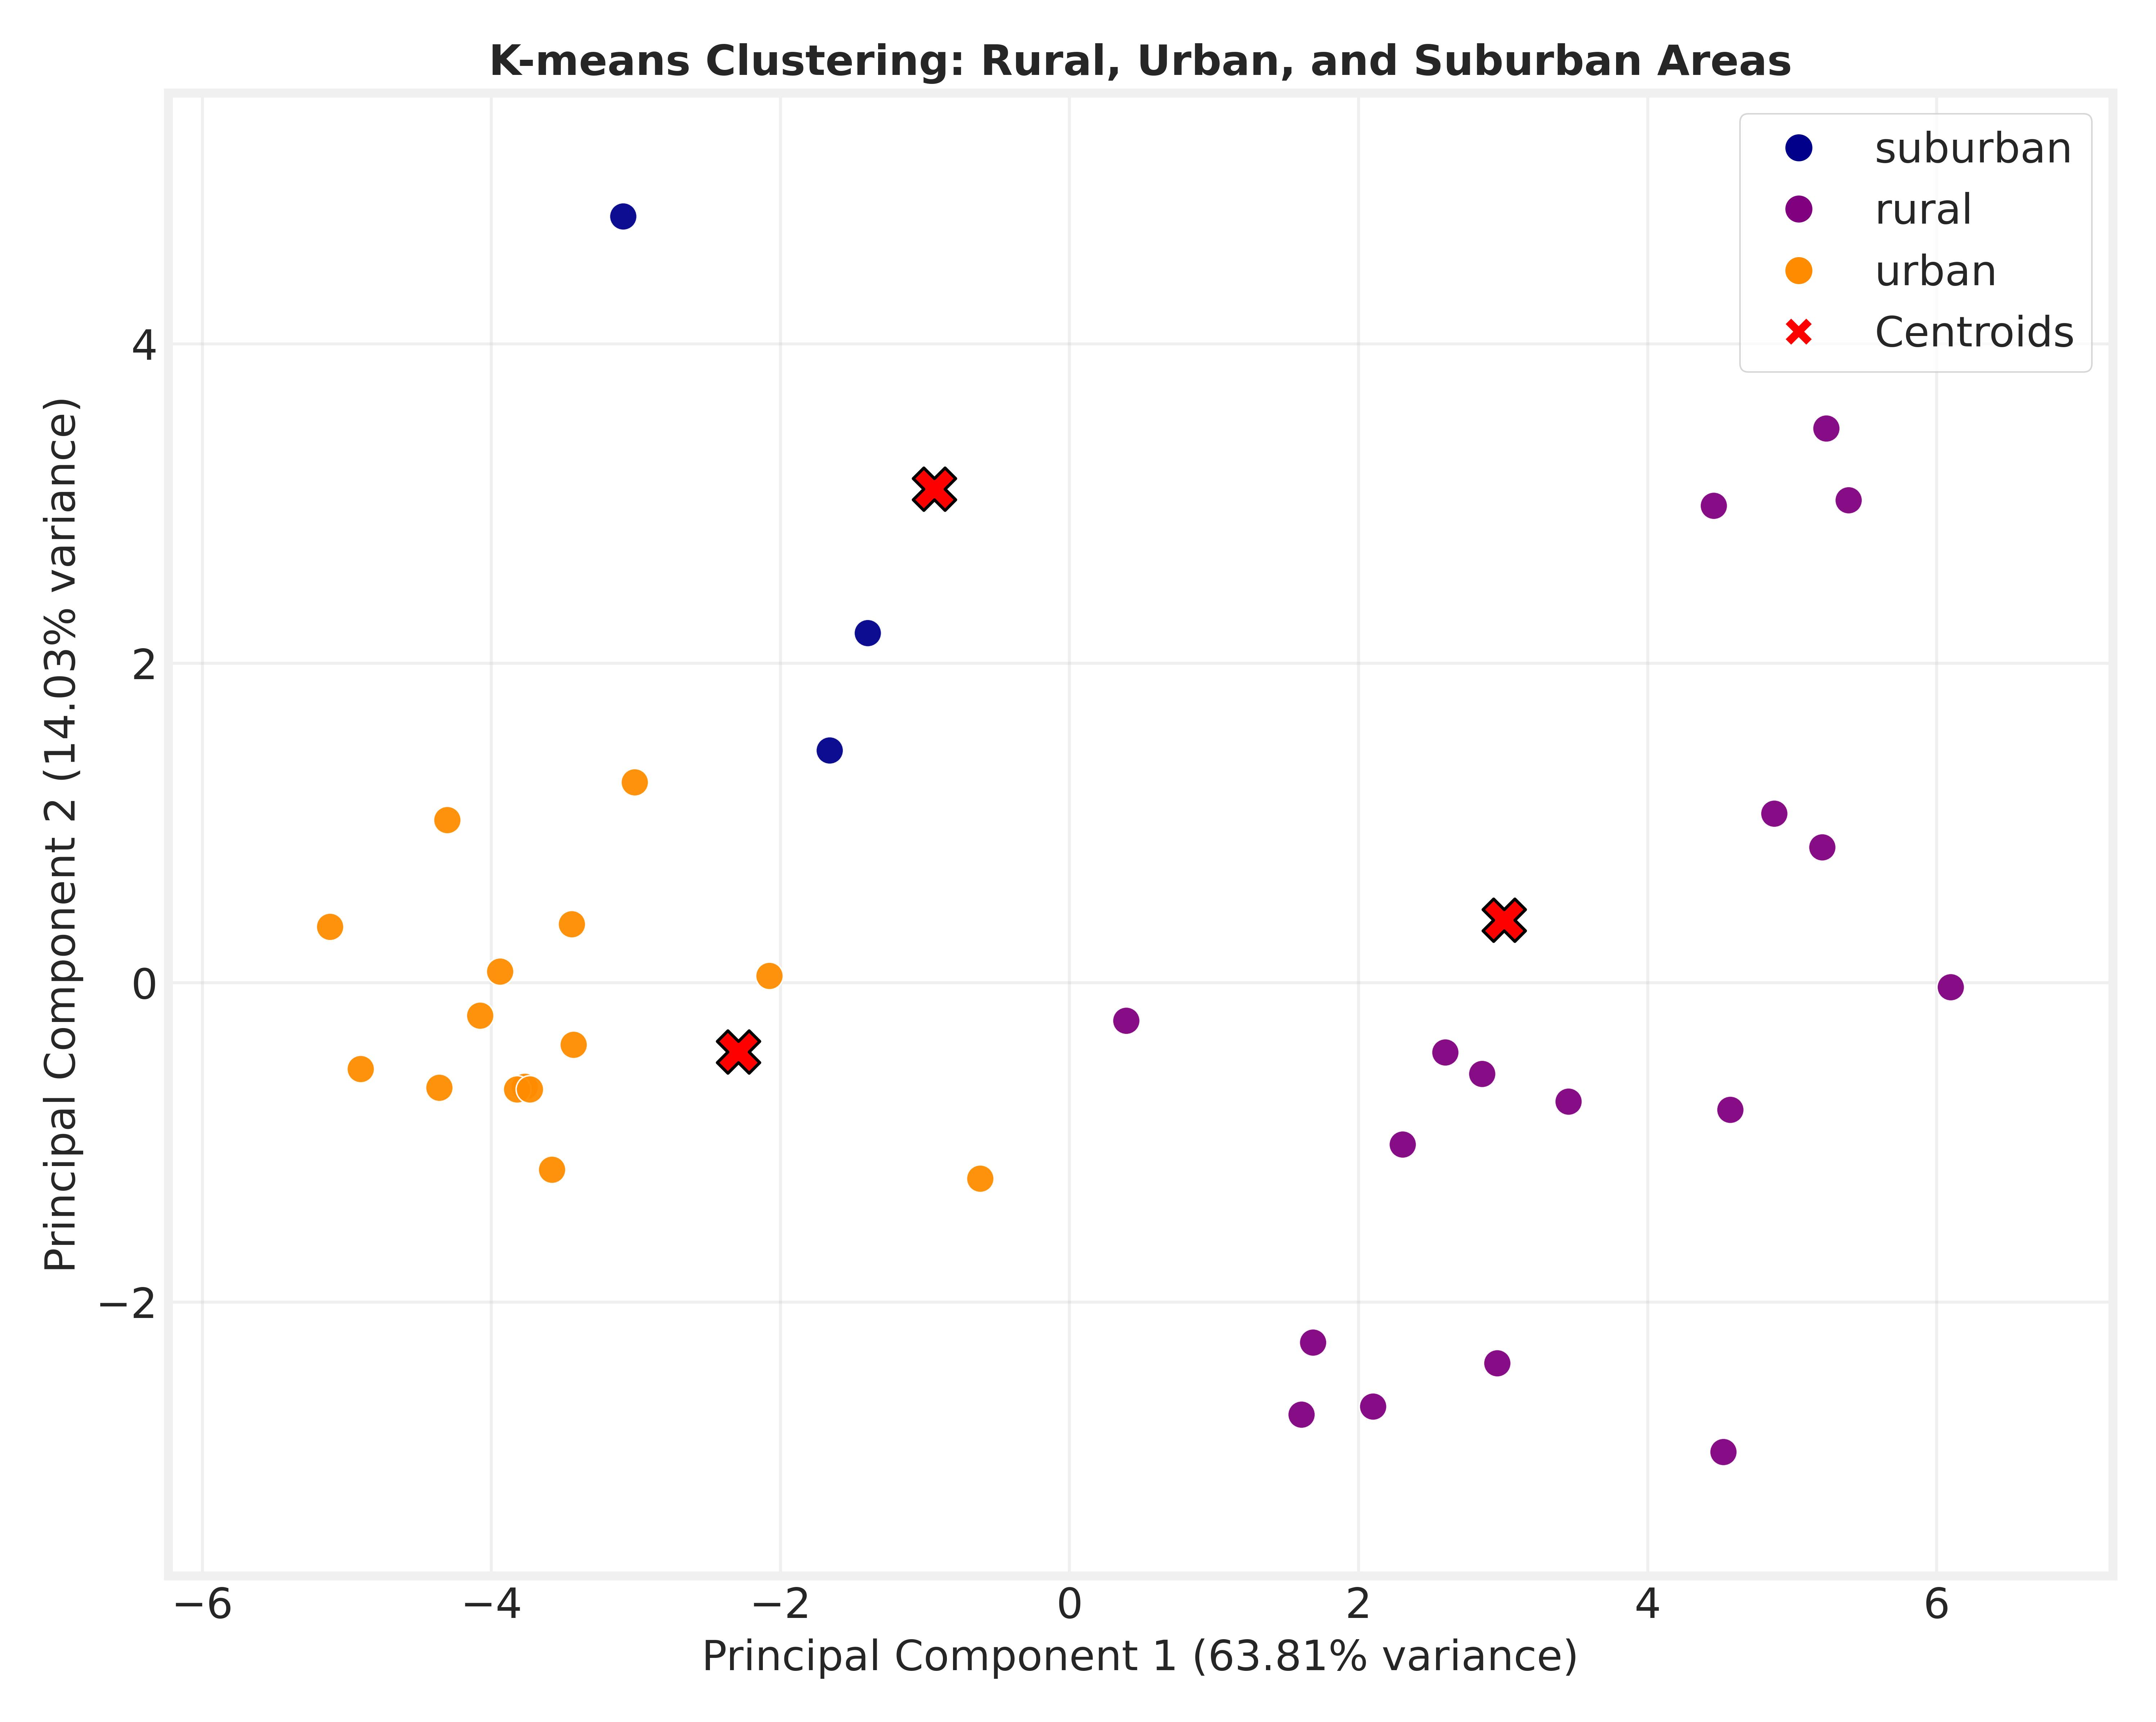
\includegraphics[width=0.47\textwidth]{figures/kmeans_clusters_1.jpg} \label{k-means_cluster1}}
    \caption{(a) Elbow method to determine the optimal number of clusters for K-means. (b) Different clusters for selected hand-labeled stations, the red points represent the centroid of different clusters.}
    \label{act_comp}
\end{figure}
\begin{table}[htb!]
\centering
\caption{Global evaluation of K-means clustering: Accuracy, Balanced accuracy, ARI-score, and NMI-score on unseen test set labeled by the TOAR data providers, as well as on the 35 Manually selected with hand-labeled classifications.}
\label{tab:kameans-main_performance}
\begin{tabular}{|lcccc|}
\hline
\textbf{~~Dataset~~} & \textbf{~~Accuracy~~} & \textbf{~~Balanced Acc.~~} & \textbf{~~ARI-score~~} & \textbf{~~NMI-score~~ } \\
\hline
35 Manually selected with hand-labels & 77.14\%  & 58.06\%  & 0.55  & 0.51  \\
35 Manually selected with TOAR labels & 77.14\%  & 58.82\%  & 0.55   & 0.546  \\
Unseen test set (1,979 stations)& 61.24\%  & 58.46\%  & 0.25  & 0.22 \\
\hline
\end{tabular}
\end{table}
\begin{table}[htb!]
\centering
\caption{Per-class evaluation of K-means clustering: Precision, recall, and F1-score on 1,979 unseen test set labeled by the TOAR data providers.}
\label{tab:kameans-perclasse_performance}
\begin{tabular}{|lcccc|}
\hline
\textbf{~~ Class ~~} & \textbf{~~Precision~~} & \textbf{~~ Recall~~} & \textbf{~~F1-score~~} & \textbf{~~Support~~ } \\
\hline
Urban & 66.83\%  & 71.88\%  & 69.26\%  & 928  \\
Suburban & 33.33\%  & 15.84\%  & 21.47\%   & 524  \\
Rural & 63.11\%  & 87.67\%  & 73.39\%  & 527 \\
\hline
\end{tabular}
\end{table}
Figure \ref{confusion_matrix_kmenas} presents the confusion matrix computed from the K-means prediction and the classes from the TOAR database as ground truth, based on 1,979  unseen test stations (see section \ref{data_method}). This confusion matrix highlights the high accuracy of K-means in classifying urban and rural stations (87.67\% and 71.88\% , respectively, see Table \ref{tab:kameans-perclasse_performance}, Recall's column). However, many instances exist where stations reported as urban or rural are classified as suburban, and vice versa. This misclassification is primarily due to the subjective nature of defining suburban areas, which often lie at the interface between rural and urban regions or exhibit a mix of urban-suburban or rural-suburban characteristics.
Additionally, Figure \ref{kmean_cluter2} visualizes the clusters defined by K-means for the 1,979  unseen test stations. 
%\textcolor{red}{ To better visualize the cluster separation, the data is projected into two dimensions using Principal Component Analysis (PCA), \citep{abdi2010principal}}. 
This visual representation clearly illustrates the fuzzy boundaries between the clusters and the noticeable spacing among the three centroids (depicted as red cross).
\begin{figure}[htb!]
    \centering
    \subfigure[]{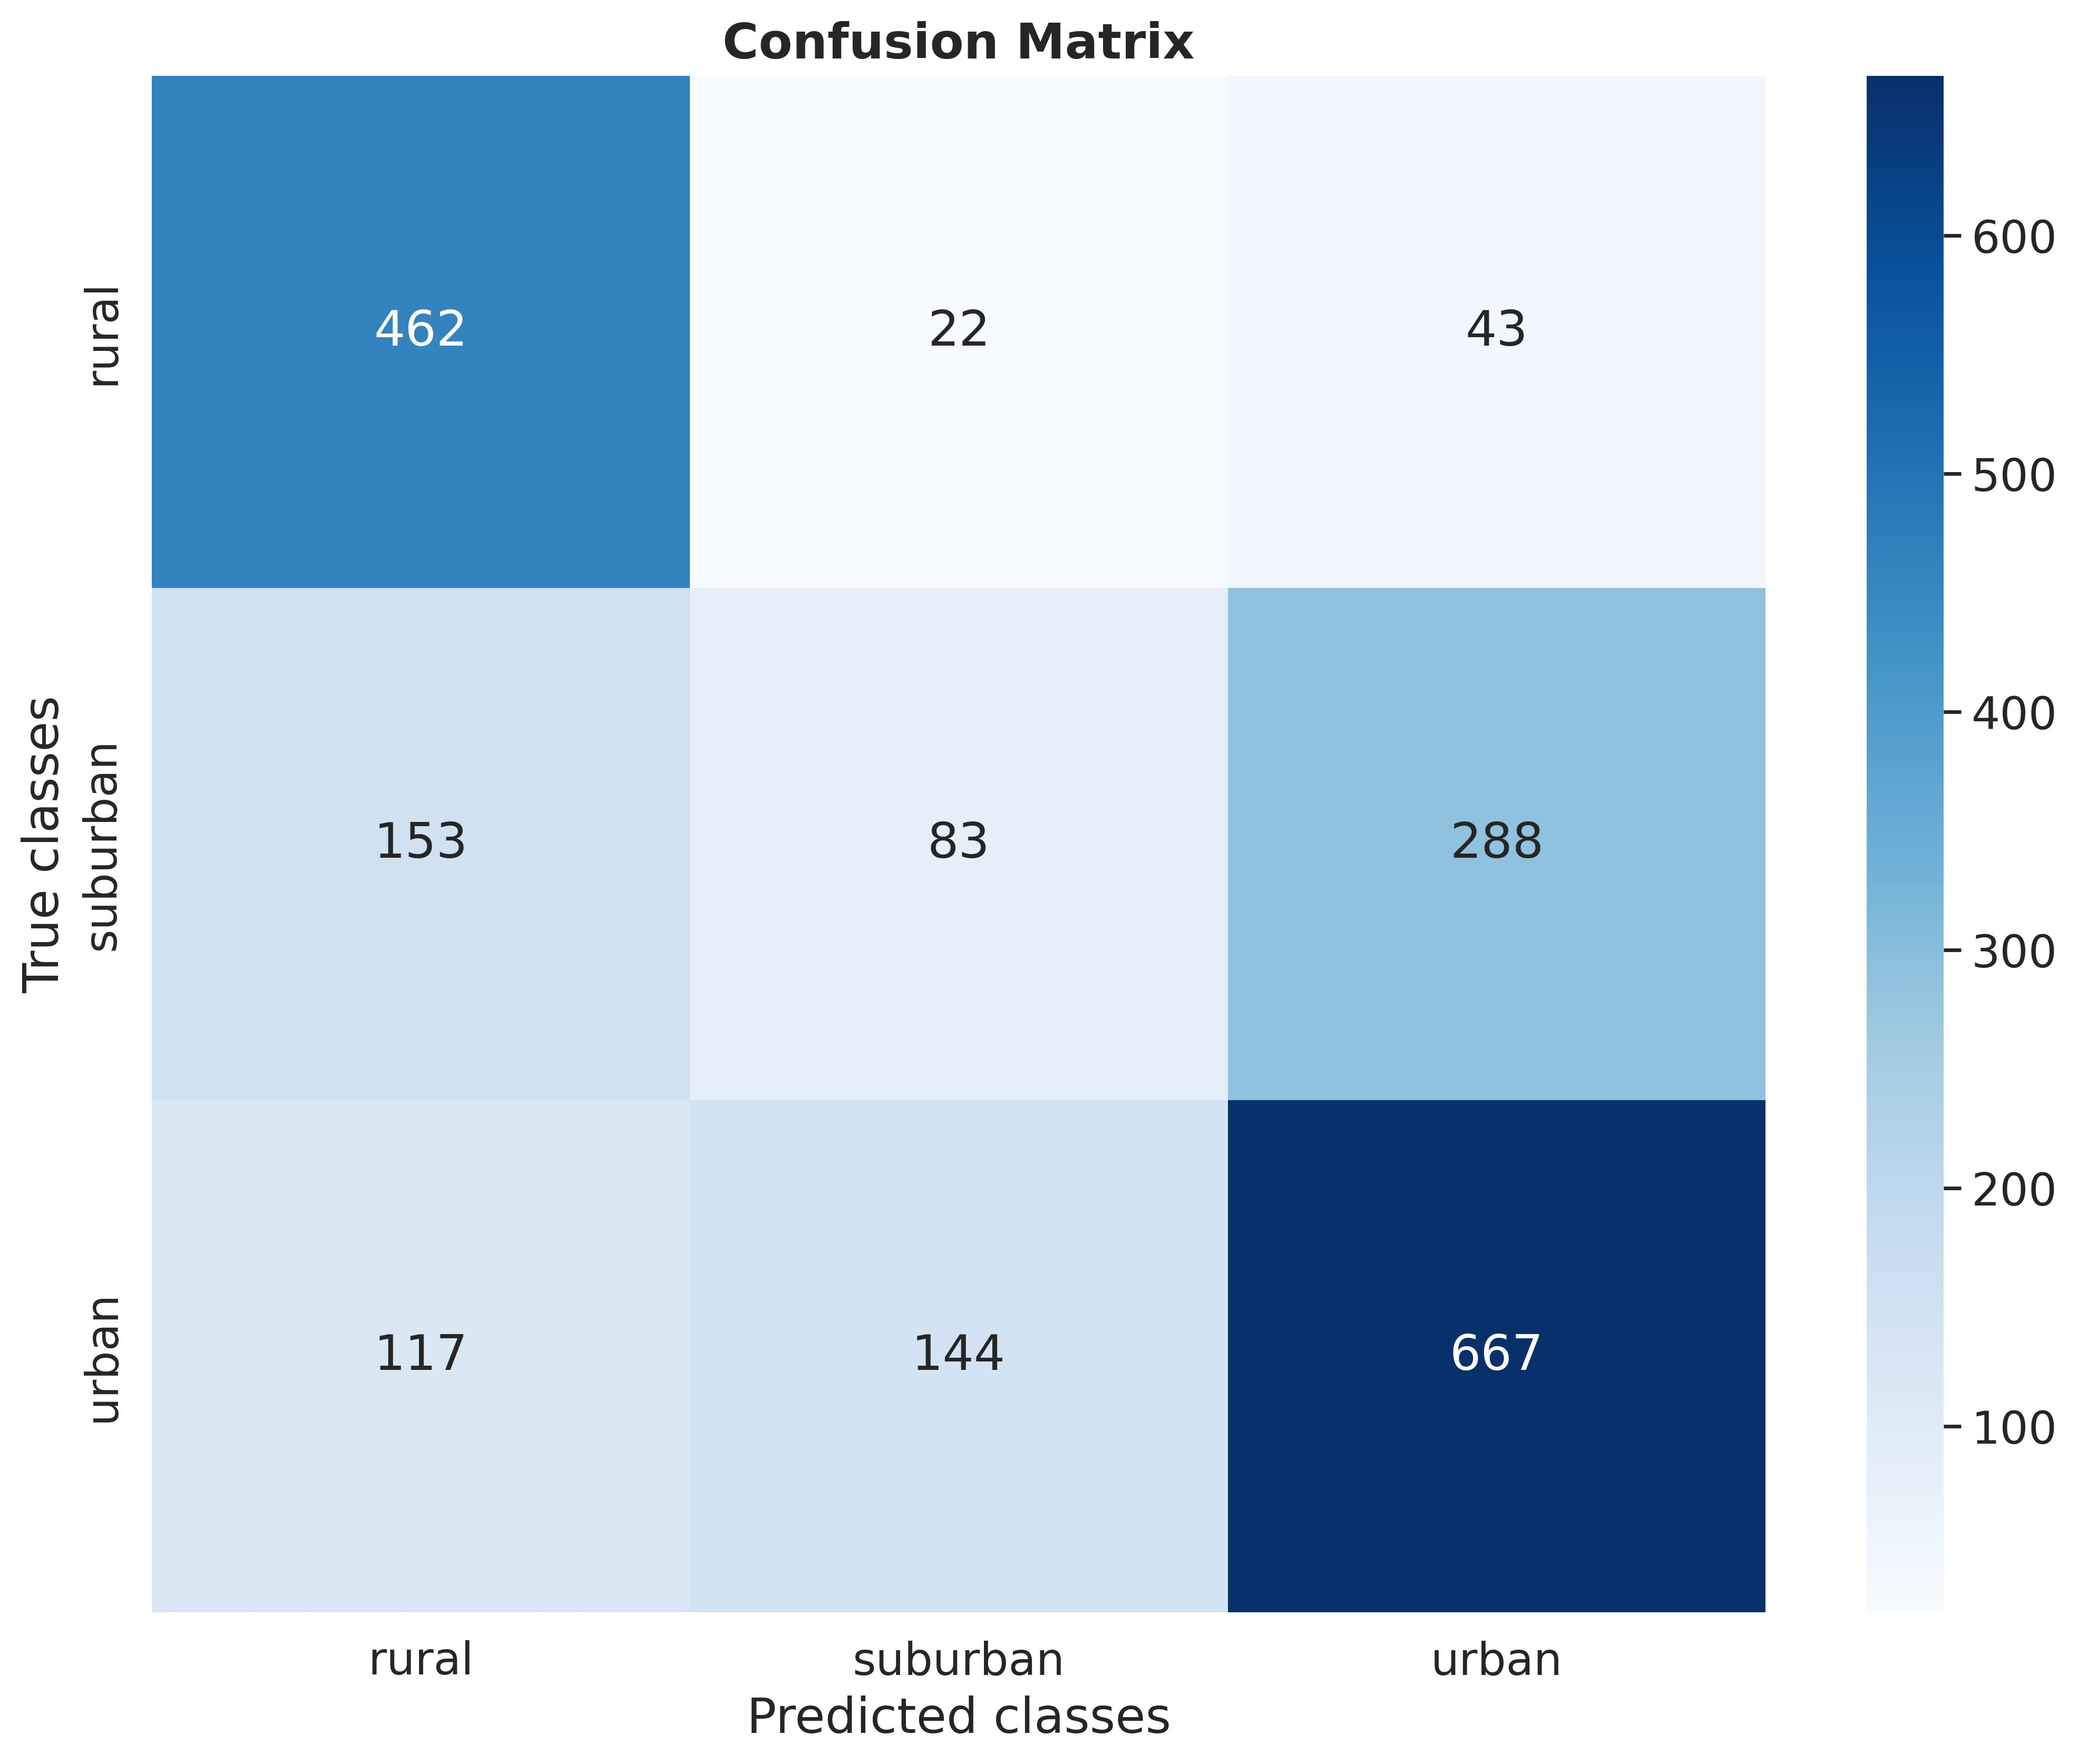
\includegraphics[width=0.468\textwidth]{figures/cm_kmean.jpg} \label{confusion_matrix_kmenas}} 
    \hskip 0.3cm
    \subfigure[]{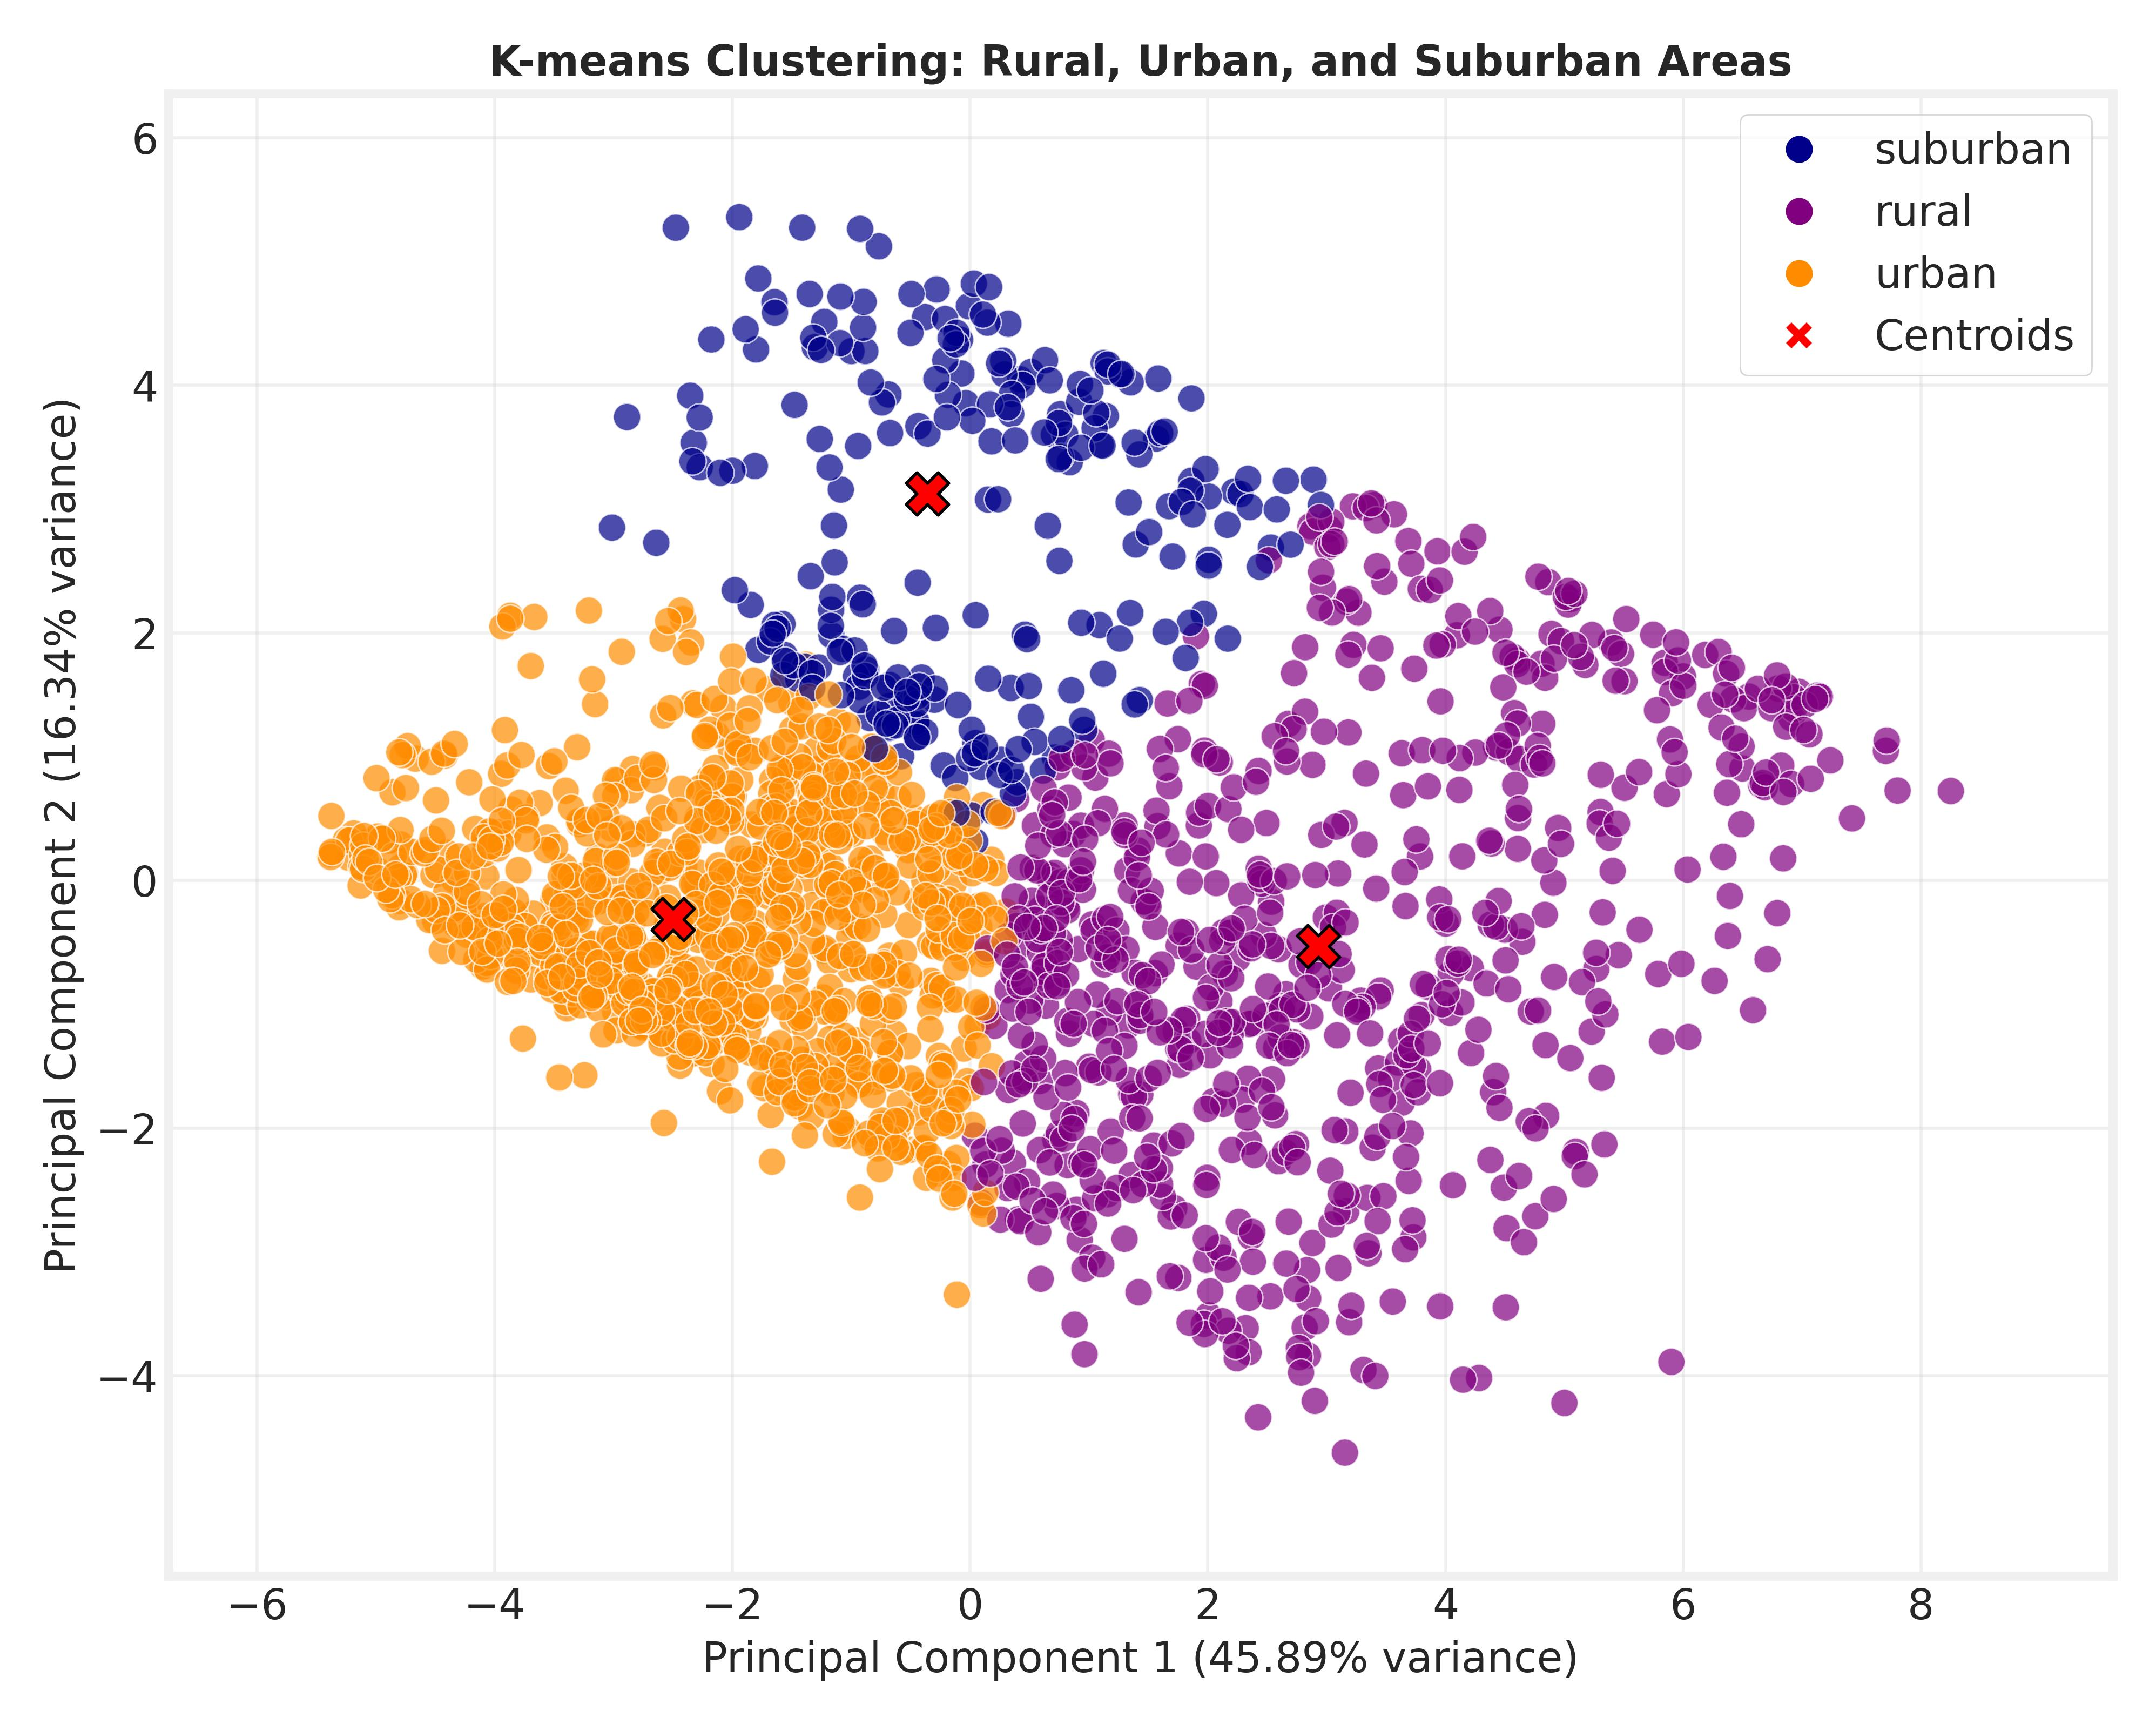
\includegraphics[width=0.5\textwidth]{figures/kmeans_clusters_2.jpg} \label{kmean_cluter2}}
    \caption{(a) Confusion matrix for K-means clustering, evaluated on 1,979  unseen labelled by the TOAR data providers. (b) Cluster visualization of the previously unseen test data.}
\end{figure}

\subsection{Results for supervised classifiers}
Here, we evaluate the results from the three supervised machine learning classifiers, Random Forest, LightGBM, and CatBoost. Furthermore, the results from the three models were subjected to a robust voting classifier to maximize the classification accuracy. We observed that the results of all algorithms are quite similar. The models demonstrated exceptional accuracy (> 83\%), high precision (> 85\%), and high F1-score (> 81 \%) in predicting urban and rural areas. However, all models struggled with the suburban class, yielding accuracies slightly above 60\% (Table~\ref{tab:supesived-perclass-perfomance_before}). As discussed above, the main reason for this lower accuracy can be attributed to the inherent subjective nature of defining this category. To address this issue, we implemented a  strategy that capitalizes on model uncertainty. By adjusting the prediction probability threshold, as detailed in Section 2, we significantly enhanced the accuracy of suburban area classifications as shown in Table~\ref{ttab:supesived-perclass-perfomance_after}. 
Figure~\ref{cm_rf} presents the confusion matrix for the Random Forest classifier and Figure~\ref{feature_importance} visualizes the feature importance. The global evaluation, i.e accuracy, balance accuracy, macro-f1 score, and weighted-f1 score of different classifiers are reported in Table~\ref{tab:supervised-main_performance_before} and Table~\ref{tab:supesived-main-perfomance_after}, which show the results before and after the probability threshold adjustment, respectively. While the overall accuracy remains relatively similar before and after the adjustment, the probability threshold adjustment significantly enhances the prediction accuracy for suburban stations, increasing it from a range of 60.85\% - 65.72\% to 66.22\%–71.95\%, and also slightly increase the F1-score for the suburban, these can be seen in details in \ref{tab:supesived-perclass-perfomance_before} and \ref{ttab:supesived-perclass-perfomance_after} presenting the per-class evaluation before and after applying the probability threshold adjustment. We also note a slight drop in accuracy when classifying urban and rural stations. However, classification performance remains high across all classifiers, with accuracy values exceeding 80\%. 
Additionally, we conducted tests on our machine learning models using the manually labeled stations, similar to those used for K-means evaluation. In this test, we found that the classifiers predict the label report on TOAR by data provider for 35 manually selected stations with 100\% accuracy and achieve an 87.88\% accuracy for the manual classified stations. 

The implementation of the adjusted probability threshold yielded notable improvements in our classification model. While the enhancements for urban and rural station predictions were modest, the impact on suburban area classification was substantial. This is particularly significant given the inherent challenges in accurately identifying suburban zones. When compared to the unsupervised K-means clustering method, our supervised approaches demonstrated superior performance across all categories. The contrast was especially pronounced in the classification of suburban areas, where K-means exhibited a markedly low accuracy of just 15.84\% , low precision of 33.33\% and low F1-score of 21.47\%, see Table~\ref{tab:kameans-perclasse_performance}. In contrast, our supervised methods achieved significantly higher accuracy rates, higher precision, and higher F1-score underscoring their effectiveness in navigating the complexities of urban-suburban-rural distinctions.

\begin{figure}[htb!]
    \centering
    \subfigure[]{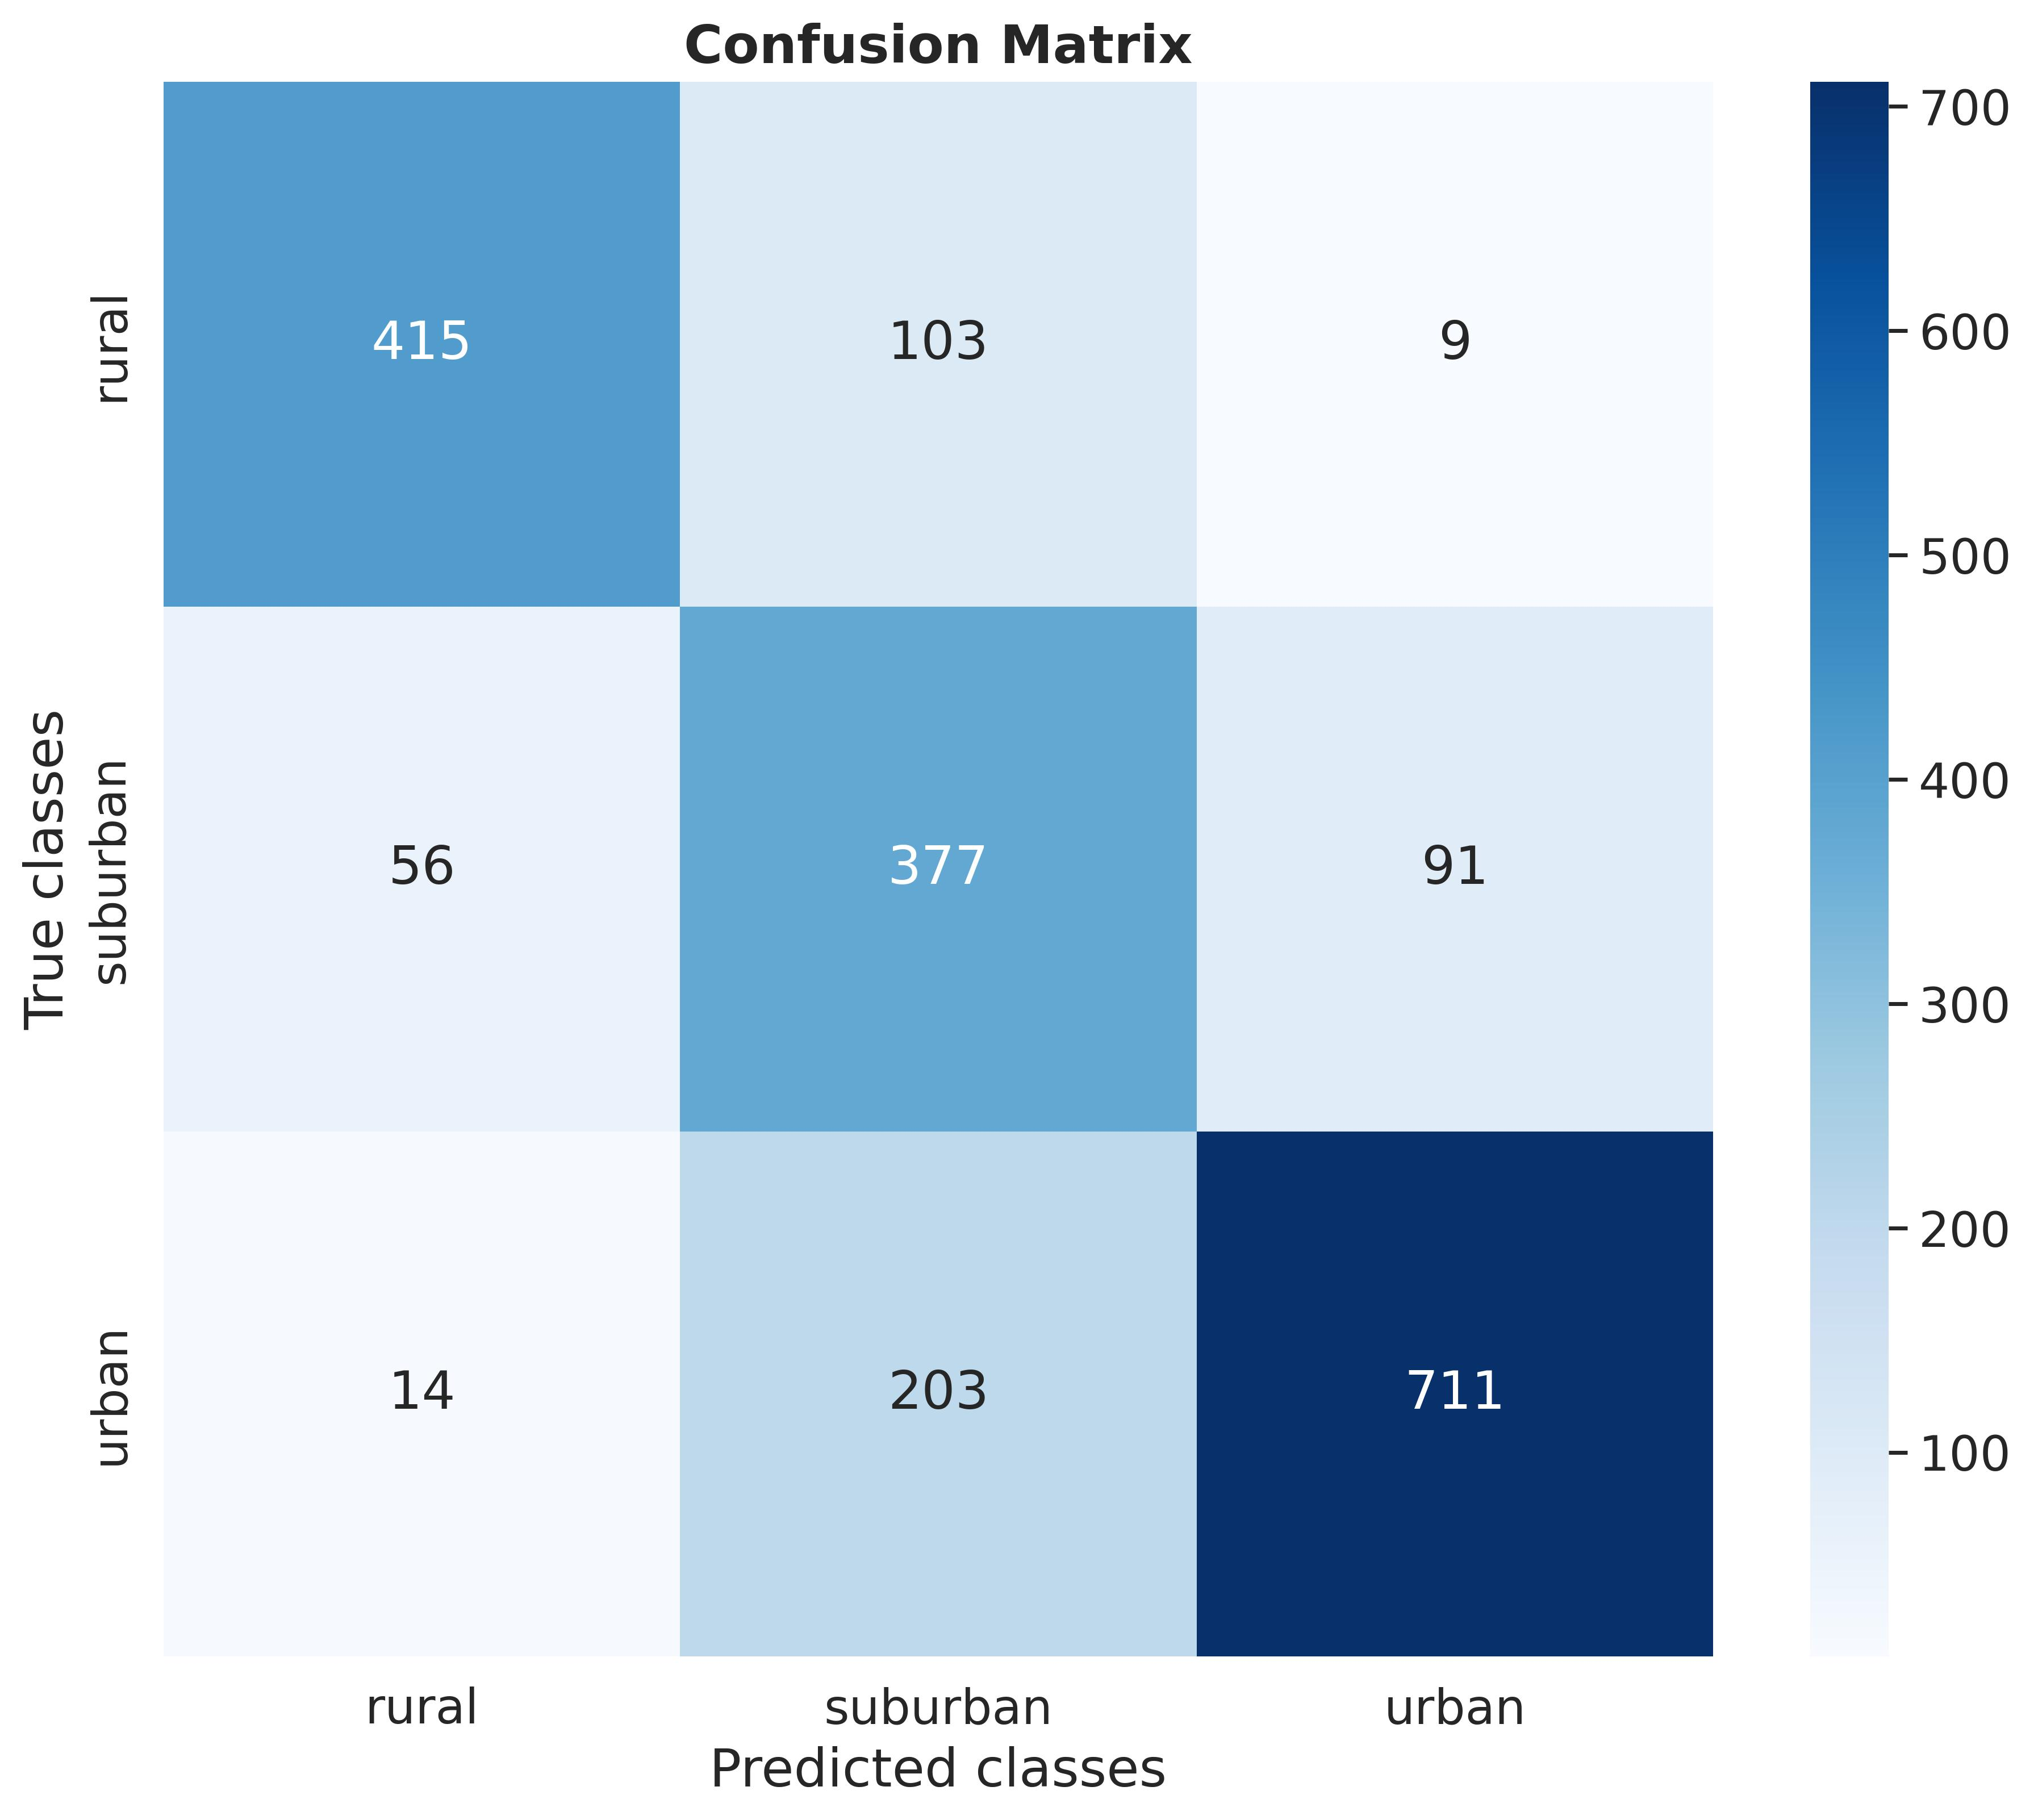
\includegraphics[width=0.45\textwidth]{figures/confusion_matrix_rf1.jpg} \label{cm_rf}} 
    \hskip 0.25cm
    \subfigure[]{\includegraphics[width=0.4999\textwidth, height=0.35\textheight]{figures/features_importances_rf_clf.jpg} \label{feature_importance}}
    \caption{(a) confusion matrix for random forest classifier, evaluated on 1,979 test data points. (b) the feature importance for random, measuring the contribution of each variable in the classification process}
\end{figure}

\begin{table}[htbp]
\centering
\caption{Global performance evaluation of models. Reported values are Accuracy, Balanced accuracy, Macro-F1 score, and Weighted-F1 score of random forest, LGBM, CatBoost, and voting classifiers before probability threshold adjustment, evaluated on 1,979 test stations.}
\label{tab:supervised-main_performance_before}
\begin{tabular}{|lcccc|}
\hline
\textbf{~~Model~~} & \textbf{~~Accuracy~~} & \textbf{~~Balanced Acc.~~} & \textbf{~~Macro-F1~~} & \textbf{~~Weighted-F1~~} \\
\hline
Random Forest& 76.25\%  & 75.39\%  & 75.07\%  & 76.53\%  \\
CatBoost & 76.25\%  & 75.70\%  & 75.27\%   & 76.66\%  \\
LightGBM & 76.81\%  & 75.54\%  & 75.42\%  & 76.93\% \\
Voting & 76.40\%  & 75.56\%  & 75.25\%  & 76.71\%  \\
\hline
\end{tabular}
\end{table}


\begin{table*}[htbp]
\centering
\caption{Per-class performance evaluation of models. Reported values are Precision, Recall, and F1 score, of random forest, LGBM, CatBoost, and voting classifiers before probability threshold adjustment, evaluated on 1,979 test stations.}
\label{tab:supesived-perclass-perfomance_before}
% Reset the counter for alphabetical labeling
\setcounter{enumi}{0}
% First row of tables
\begin{minipage}[t]{0.25\textwidth}
\centering
\alphcaption{Random Forest}\\
\vspace{0.5em}
\begin{tabular}{|lcccc|}
\toprule
\textbf{Class} & \textbf{Precision} & \textbf{Recall} & \textbf{F1-score} & \textbf{Support} \\
\midrule
Urban & 85.02\%  &  79.53\%  &  82.18\%   &    928 \\
Suburban & 57.74\%  &  63.36\%  &  60.42\%    &   524 \\
Rural & 81.90\%  &  83.30\%  &  82.60\%    &   527 \\
\bottomrule
\end{tabular}
\end{minipage}
\hfill
\begin{minipage}[t]{0.55\textwidth}
\centering
\alphcaption{CatBoost}\\
\vspace{0.5em}
\begin{tabular}{|lcccc|}
\toprule
\textbf{Class} & \textbf{Precision} & \textbf{Recall} & \textbf{F1-score} & \textbf{Support}\\
\midrule
Urban & 86.04\%  &  78.34\%  &  82.01\%    &   928 \\
Suburban & 57.00\%  &  65.27\%  &  60.85\%   &    524 \\
Rural & 82.40\% &   83.49\%  &  82.94\%   &    527 \\
\bottomrule
\end{tabular}
\end{minipage}

\vspace{1.em} % Vertical space between rows

% Second row of tables
\begin{minipage}[t]{0.25\textwidth}
\centering
\alphcaption{LightGBM}\\
\vspace{0.5em}
\begin{tabular}{|lcccc|}
\toprule
\textbf{Class} & \textbf{Precision} & \textbf{Recall} & \textbf{F1-score} & \textbf{Support} \\
\midrule
Urban & 83.85\%  &  81.68\%  &  82.75\%  &     928 \\
Suburban & 59.16\%  &  61.64\%  &  60.37\%   &    524 \\
Rural & 82.99\%  &  83.30\%  &  83.14\%    &   527 \\
\bottomrule
\end{tabular}
\end{minipage}
\hfill
\begin{minipage}[t]{0.55\textwidth}
\centering
\alphcaption{Voting}\\
\vspace{0.5em}
\begin{tabular}{|lcccc|}
\toprule
\textbf{Class} & \textbf{Precision} & \textbf{Recall} & \textbf{F1-score} & \textbf{Support} \\
\midrule
Urban & 85.24\%  &  79.63\%  &  82.34\%  &     928 \\
Suburban & 57.59\%  &  63.74\% &  60.51\%   &    524 \\
Rural & 82.52\%  &  83.30\%  &  82.91\%   &    527 \\
\bottomrule
\end{tabular}
\end{minipage}
\end{table*}



\begin{table}[htb!]
\centering
\caption{Global performance evaluation of models. Reported values are Accuracy, Balanced accuracy, Macro-F1 score, and Weighted-F1 score of random forest, LGBM, CatBoost, and voting classifiers after applying probability threshold adjustment, evaluated on 1,979 test stations.}
\label{tab:supesived-main-perfomance_after}
\begin{tabular}{|lcccc|}
\hline
\textbf{~~Model~~} & \textbf{~~Accuracy~~} & \textbf{~~Balanced Acc.~~} & \textbf{~~Macro-F1~~} & \textbf{~~Weighted-F1~~ } \\
\hline
Random Forest& 75.95\%  & 75.77\%  & 75.42\%  & 76.73\%  \\
CatBoost & 76.30\%  & 75.85\%  & 75.40\%   & 76.74\%  \\
LightGBM & 76.96\%  & 76.20\%  & 76.04\%  & 77.36\% \\
Voting & 76.50\%  & 76.10\%  & 75.79\%  & 77.07\%  \\
\hline
\end{tabular}
\end{table}

% \begin{table}[htb!]
% \centering
% \caption{Accuracy of random forest, LGBM, CatBoost, and voting classifiers before probability threshold adjustment, evaluated on 1,000 test stations.}
% \begin{tabular}{l|l|l|l|l|}
% \cline{2-5} & \textbf{Random forest} & \textbf{CatBoost} & \textbf{LGBM} & \textbf{Voting} \\ \hline
% \multicolumn{1}{|l|}{Global Accuracy} & \textbf{$79.01$\%}  & $77.50$\%  & $76.20$\%  & $78.70$\%  \\ \hline
% \multicolumn{1}{|l|}{Accuracy for urban}    & \textbf{$91.03$\%}      & $88.28$\%  & $88.05$\% & $90.80$\%   \\ \hline
% \multicolumn{1}{|l|}{Accuracy for rural}    & $86.64$\%   & \textbf{$84.12$\%}   & $83.03$\% & \textbf{$84.84$\%} \\ \hline
% \multicolumn{1}{|l|}{Accuracy for suburban} & $53.47$\%   & \textbf{$54.86$\%}   & $51.74$\% & $54.51$\%   \\ \hline
% \end{tabular}
% \label{supervized_results_before_prob_adj}
% \end{table}

% \begin{table}[htb!]
% \centering
% \caption{Accuracy of random forest, LGBM, CatBoost, and voting classifiers after probability threshold adjustment, evaluated on 1,000 test stations.}
% \begin{tabular}{l|l|l|l|l|}
% \cline{2-5} & \textbf{Random forest} & \textbf{CatBoost} & \textbf{LGBM} & \textbf{Voting} \\ \hline
% \multicolumn{1}{|l|}{Global Accuracy} & \textbf{$76.90$\%}  & $77.10$\%  & $77.50$\%  & $78.20$\%  \\ \hline
% \multicolumn{1}{|l|}{Accuracy for urban}    & \textbf{$82.93$\%}      & $83.15$\%  & $85.56$\% & $84.90$\%   \\ \hline
% \multicolumn{1}{|l|}{Accuracy for rural}    & $80.85$\%   & \textbf{$81.21$\%}   & $82.27$\% & \textbf{$82.27$\%} \\ \hline
% \multicolumn{1}{|l|}{Accuracy for suburban} & $62.07$\%   & \textbf{$62.07$\%}   & $58.24$\% & $62.07$\%   \\ \hline
% \end{tabular}
% \label{supervized_results_after_prob_ad}
% \end{table}

% \begin{table*}[htbp]
% \centering
% \caption{Performance metrics for different experimental settings.}
% \label{tab:all_results}
% % First row of tables
% \begin{minipage}[t]{0.2\textwidth}
% \centering
% \caption{Random Forest}
% \begin{tabular}{|lcccc|}
% \toprule
% \textbf{Class} & \textbf{Precision} & \textbf{Recall} & \textbf{F1-score} & \textbf{Support} \\
% \midrule
% Urban & 87.67\% &   76.62\%  & 81.77\%   &    928 \\
% Suburban & 55.20\%  &  71.95\%  &  62.47\%   &    524 \\
% Rural & 85.57\% &   78.75\% &   82.02\%   &    527 \\
% \bottomrule
% \end{tabular}
% \end{minipage}
% \hfill
% \begin{minipage}[t]{0.49\textwidth}
% \centering
% \caption{CatBoost}
% \begin{tabular}{|lcccc|}
% \toprule
% \textbf{Class} & \textbf{Precision} & \textbf{Recall} & \textbf{F1-score} & \textbf{Support}\\
% \midrule
% Urban & 86.29\%  &  78.02\%  &  81.95\%   &    928 \\
% Suburban & 56.98\%  &  66.22\%  &  61.25\%    &   524 \\
% Rural &  82.67\% &   83.30\%  &  82.99\%   &    527 \\
% \midrule
% %\bottomrule
% \end{tabular}
% \end{minipage}

% \vspace{1.em} % Vertical space between rows
% % Second row of tables
% \begin{minipage}[t]{0.2\textwidth}
% \centering
% \caption{LightGBM}
% \begin{tabular}{|lcccc|}
% \toprule
% \textbf{Class} & \textbf{Precision} & \textbf{Recall} & \textbf{F1-score} & \textbf{Support} \\
% \midrule
% Urban & 85.27\%  &  79.85\%  &  82.47\%   &    928 \\
% Suburban & 57.90  &  66.41\% &   61.87\%   &    524 \\
% Rural & 85.27\% &   82.35\%  &  83.78\%   &    527 \\
% \midrule
% %\bottomrule
% \end{tabular}
% \end{minipage}
% \hfill
% \begin{minipage}[t]{0.49\textwidth}
% \centering
% \caption{Voting}
% \begin{tabular}{|lcccc|}
% \toprule
% \textbf{Class} & \textbf{Precision} & \textbf{Recall} & \textbf{F1-score} & \textbf{Support} \\
% \midrule
% Urban & 86.55\%  &  78.34\%  &  82.24\%   &    928
%  \\
% Suburban & 56.80\%  &  68.51\%  &  62.11\%   &    524 \\
% Rural & 85.01\%  &  81.78\%  &  83.37\%  &     527 \\
% \midrule
% %\bottomrule
% \end{tabular}
% \end{minipage}
% \end{table*}

% \begin{table}[htbp]
% \centering
% \caption{Classification performance per class with macro- and micro-averages and balanced accuracy.}
% \label{tab:classification_metrics}
% \begin{tabular}{|lcccc|}
% \hline
% \textbf{Class} & \textbf{Precision} & \textbf{Recall} & \textbf{F1-score} & \textbf{Support} \\
% \hline
% Urban & 0.91 & 0.88 & 0.89 & 120 \\
% Suburban & 0.84 & 0.86 & 0.85 & 150 \\
% Rural & 0.79 & 0.75 & 0.77 & 130 \\
% \hline
% \textbf{Macro Avg} & 0.85 & 0.83 & 0.84 & -- \\
% \textbf{Micro Avg} & 0.86 & 0.86 & 0.86 & 400 \\
% \textbf{Balanced Accuracy} & -- & -- & -- & 0.83 \\
% \hline
% \end{tabular}

% \end{table}

\begin{table*}[htbp]
\centering
\caption{Per-class performance evaluation of models. Reported values are Precision, Recall, and F1 score, of random forest, LGBM, CatBoost, and voting classifiers after applying probability threshold adjustment, evaluated on 1,979 test stations.}
\label{ttab:supesived-perclass-perfomance_after}

% Reset the counter for alphabetical labeling
\setcounter{enumi}{0}

% First row of tables
\begin{minipage}[t]{0.25\textwidth}
\centering
\alphcaption{Random Forest}\\
\vspace{0.5em}
\begin{tabular}{|lcccc|}
\toprule
\textbf{Class} & \textbf{Precision} & \textbf{Recall} & \textbf{F1-score} & \textbf{Support} \\
\midrule
Urban & 87.67\% &   76.62\%  & 81.77\%   &    928 \\
Suburban & 55.20\%  &  71.95\%  &  62.47\%   &    524 \\
Rural & 85.57\% &   78.75\% &   82.02\%   &    527 \\
\bottomrule
\end{tabular}
\end{minipage}
\hfill
\begin{minipage}[t]{0.55\textwidth}
\centering
\alphcaption{CatBoost}\\
\vspace{0.5em}
\begin{tabular}{|lcccc|}
\toprule
\textbf{Class} & \textbf{Precision} & \textbf{Recall} & \textbf{F1-score} & \textbf{Support}\\
\midrule
Urban & 86.29\%  &  78.02\%  &  81.95\%   &    928 \\
Suburban & 56.98\%  &  66.22\%  &  61.25\%    &   524 \\
Rural &  82.67\% &   83.30\%  &  82.99\%   &    527 \\
\bottomrule
\end{tabular}
\end{minipage}

\vspace{1.em} % Vertical space between rows

% Second row of tables
\begin{minipage}[t]{0.25\textwidth}
\centering
\alphcaption{LightGBM}\\
\vspace{0.5em}
\begin{tabular}{|lcccc|}
\toprule
\textbf{Class} & \textbf{Precision} & \textbf{Recall} & \textbf{F1-score} & \textbf{Support} \\
\midrule
Urban & 85.27\%  &  79.85\%  &  82.47\%   &    928 \\
Suburban & 57.90\%  &  66.41\% &   61.87\%   &    524 \\
Rural & 85.27\% &   82.35\%  &  83.78\%   &    527 \\
\bottomrule
\end{tabular}
\end{minipage}
\hfill
\begin{minipage}[t]{0.55\textwidth}
\centering
\alphcaption{Voting}\\
\vspace{0.5em}
\begin{tabular}{|lcccc|}
\toprule
\textbf{Class} & \textbf{Precision} & \textbf{Recall} & \textbf{F1-score} & \textbf{Support} \\
\midrule
Urban & 86.55\%  &  78.34\%  &  82.24\%   &    928 \\
Suburban & 56.80\%  &  68.51\%  &  62.11\%   &    524 \\
Rural & 85.01\%  &  81.78\%  &  83.37\%  &     527 \\
\bottomrule
\end{tabular}
\end{minipage}
\end{table*}

\subsection{Discussion}
The supervised machine learning approach demonstrates remarkable performance, achieving prediction accuracies > 84\% for urban and rural stations when applied to previously unseen test data. This can already be used to accurately predict "urban" and "rural" labels.  While the model's performance in identifying suburban areas initially showed slightly lower accuracy, this challenge was effectively addressed through the adjusted probability threshold. 

Despite the promising results, the classification results are far from perfect. This can be partially attributed to inherent inaccuracies within the dataset itself. To investigate this issue, we conducted a detailed review and manual inspection of the 30   randomly selected misclassifications. For these stations, which are listed in Table~\ref{mis_class}, we visually inspected the areas around the stations on Google Maps \cite{mehta2019google}, using a zoom level of 11 or greater. While 6 of these cases revealed wrong classifications by our best ML model, the model's classification is actually more accurate than the label that was reported by the data providers in 16  cases. In the remaining 8 cases, neither the reported nor the ML model derived label was correct. In one of these cases, both the reported and ML based label was urban, while the station site is apparently located in a rural area. In the other case, visual inspection would place the station in the suburban class, while the reported category is urban and the ML model classifies the station as rural. However, for stations misclassified by our machine learning model, we observed ambiguous features that could misguide our model. For instance, surrounding neighborhoods of areas reported as urban but classified as rural by our model exhibited rural characteristics, such as lower population density (which is one of the important features used in the training dataset, see Figure~\ref{feature_importance}) and more green space. This result, while initially counter-intuitive, can be explained by the strong robustness of tree-based ensemble methods to noisy datasets. Algorithms such as Random Forest, CatBoost, and LightGBM are specifically designed to mitigate the effects of noise and outliers through randomization and averaging techniques \citep{biau2016random}. However, these 30 data points are insufficient to draw definitive conclusions. 

 \begin{table}[htb!]
\centering
\caption{Closer analysis of some misclassified station locations}
\begin{tabular}{|r|r|r|r|r|r|r|}
\hline
latitude  & longitude&   Station code &   type of area TOAR & type of area ML & \makecell{True type of area \\ (From Google Maps)} & ~~~~Winner \\ \hline
\textbf{33.859662} & \textbf{−118.200707} & 06-037-4008  & suburban       & urban           & urban             & ML     \\ \hline
\textbf{44.470336} & \textbf{−71.180077}&  33-007-0015   & urban             & suburban           & rural          & None   \\ \hline
\textbf{53.341875} & \textbf{−6.214075}&  IE004AP  & urban             & rural           & rural             & ML     \\ \hline
\textbf{42.876469} & \textbf{-73.071215}& 50-003-0001 & urban             & rural           & rural             & ML     \\ \hline
\textbf{44.307000} & \textbf{-86.242649}& 26-101-0922 & urban             & rural           & rural             & ML     \\ \hline
\textbf{52.132417} & \textbf{-0.300306}& GB0954A & urban             & suburban          & suburban         & ML     \\ \hline
\textbf{44.835700} & \textbf{-108.386000}& 56-003-0003 & rural             & suburban           & rural          & TOAR   \\ \hline
\textbf{35.273460} & \textbf{-89.961217}& 47-157-0046 & suburban             & rural       & urban             & None   \\ \hline
\textbf{40.734449} & \textbf{-75.312389}& 42-095-1000	  & urban             & suburban           & suburban      & ML   \\ \hline
\textbf{45.394410} & \textbf{-93.885254}& 27-141-0012	& urban             & rural        & suburban             & None     \\ \hline
\textbf{36.923100} & \textbf{-2.463220}& 04024001 & urban             & suburban        & suburban           & ML     \\ \hline
\textbf{44.390480} & \textbf{8.201500}& IT1233A	 & rural             & suburban        & suburban             & ML   \\ \hline
\textbf{48.762780} & \textbf{-122.440280}&  53-073-0015  & suburban            & urban        & rural             & None   \\ \hline
\textbf{50.575364} & \textbf{8.492018}& DEHE095 & suburban            & urban          & urban                & ML   \\ \hline
\textbf{30.958515} & \textbf{-88.028332}& 01-097-0028 & suburban             & rural       & rural           & ML     \\ \hline
\textbf{31.813370} & \textbf{-106.464520}&  48-141-0693  & urban            & suburban     & suburban          & ML     \\ \hline
\textbf{37.049260} & \textbf{-86.214870}& 21-227-0009  & suburban             & rural        & rural          & ML     \\ \hline
\textbf{43.629605} & \textbf{-72.309499}& 33-009-0010 & urban          & rural           & rural              & ML   \\ \hline
\textbf{40.262540} & \textbf{-89.230923}& 17-107-0001  & urban          & suburban           & rural             & None   \\ \hline
\textbf{33.089772} & \textbf{-87.459733}& 01-125-0010  & suburban          & rural           & rural          & ML   \\ \hline
\textbf{44.003853} & \textbf{-92.414896}& 27-109-0016 & rural          & suburban           & rural             & TOAR     \\ \hline
\textbf{39.652473} & \textbf{-104.925926}& 08-031-0823 & urban          & suburban           & suburban          & ML  \\ \hline
\textbf{47.689728} & \textbf{22.458500}& RO0183A & suburban          & urban          & suburban          & TOAR   \\ \hline
\textbf{43.144070} & \textbf{-2.963370}& 01036004  & suburban             & urban        & suburban          & TOAR     \\ \hline
\textbf{32.891056} & \textbf{-111.570503}& 04-021-3011 & suburban          & rural           & suburban              & TOAR  \\ \hline
\textbf{40.246528} & \textbf{-77.186750}& 42-041-0101  & rural          & suburban           & rural             & TOAR   \\ \hline
\textbf{60.294268} & \textbf{5.324619}& NO0121A  & suburban          & urban           & rural          & None   \\ \hline
\textbf{57.039915} & \textbf{-135.272042}& 02-220-0007	 & suburban          & rural           & rural             & ML     \\ \hline
\textbf{62.486778} & \textbf{17.324437}& SE0012A & urban          & suburban           & rural          & None \\ \hline
\textbf{38.583226} & \textbf{-77.121900}& 11-001-0025 & urban          & rural          & suburban          & None   \\ \hline
\end{tabular}
\label{mis_class}
\end{table}

% \begin{table}[htb!]
% \centering
% \caption{Closer analysis of some misclassified station locations}
% \begin{tabular}{|r|r|r|r|r|r|}
% \hline
% latitude           & longitude            & type of area TOAR & type of area ML & True type of area (From Google Maps)& ~~~~Winner \\ \hline
% \textbf{59.123314} & \textbf{ 11.391136}   & rural             & urban           & urban             & ML     \\ \hline
% \textbf{34.985670} & \textbf{-84.375193}  & urban             & rural           & suburban          & None   \\ \hline
% \textbf{34.710100} & \textbf{128.587500}  & urban             & rural           & rural             & ML     \\ \hline
% \textbf{37.360500} & \textbf{128.125600}  & urban             & rural           & rural             & ML     \\ \hline
% \textbf{41.285533} & \textbf{-93.583983}  & urban             & rural           & rural             & ML     \\ \hline
% \textbf{44.785616} & \textbf{-69.885058}  & urban             & rural           & rural             & ML     \\ \hline
% \textbf{35.102638} & \textbf{-85.162194}  & urban             & rural           & urban             & TOAR   \\ \hline
% \textbf{45.542222} & \textbf{9.516389}    & urban             & suburban        & suburban          & ML     \\ \hline
% \textbf{39.720451} & \textbf{-94.872693}  & urban             & suburban        & urban             & TOAR   \\ \hline
% \textbf{48.691113} & \textbf{21.286388}   & urban             & urban           & rural             & None   \\ \hline
% \textbf{35.259502} & \textbf{-120.644720} & urban             & suburban        & suburban          & ML     \\ \hline
% \textbf{37.049115} & \textbf{-122.019962} & urban             & suburban        & suburban          & ML     \\ \hline
% \textbf{41.895812} & \textbf{-87.607683}  & urban             & suburban        & urban             & TOAR   \\ \hline
% \textbf{41.193587} & \textbf{1.236703}    & rural             & suburban        & rural             & TOAR   \\ \hline
% \textbf{34.131714} & \textbf{-109.282309} & rural             & suburban        & rural             & TOAR   \\ \hline
% \textbf{33.061150} & \textbf{-112.052040} & rural             & suburban        & suburan           & ML     \\ \hline
% \textbf{49.076550} & \textbf{8.406660}    & rural             & suburban        & suburban          & ML     \\ \hline
% \textbf{36.186210} & \textbf{-5.380810}   & rural             & suburban        & suburban          & ML     \\ \hline
% \textbf{45.647310} & \textbf{13.854970}   & rural             & suburban        & suburban          & ML     \\ \hline
% \textbf{43.045269} & \textbf{-70.713958}  & suburban          & rural           & suburban          & TOAR   \\ \hline
% \textbf{44.013056} & \textbf{12.420000}   & suburban          & rural           & rural             & ML     \\ \hline
% \textbf{43.186600} & \textbf{-8.471600}   & suburban          & rural           & suburban          & TOAR   \\ \hline
% \textbf{36.587027} & \textbf{-89.546742}  & suburban          & rural           & rural             & ML     \\ \hline
% \textbf{40.077780} & \textbf{-6.147220}   & suburban          & rural           & rural             & ML     \\ \hline
% \textbf{35.498711} & \textbf{-83.310242}  & suburban          & rural           & suburban          & TOAR   \\ \hline
% \end{tabular}
% \label{mis_class}
% \end{table}

%\textcolor{B}{L230: Use of pollutant concentrations. The evaluation with NOx and PM2.5 is a useful plausibility check. However, the choice of the 75th percentile is not self-evident. Please justify why the 75th percentile was chosen (e.g., is this a standard in this field or intended to capture robustly elevated concentrations while avoiding sensitivity to extremes?).}

To further lend confidence to our results, we evaluated the 75-percentile statistics of the primary air pollutant concentrations NO$_x$ and PM$_{2.5}$ from the TOAR database. We chose the 75-th percentile, because urban areas typically exhibit fresh pollution with many high concentration events. This percentile  captures such characteristics while being more robust than either the maximum value or a higher percentile. While data on these species is incomplete, there are sufficient measurements from several regions to yield a meaningful statistic. Figure~\ref{nox_pm_eval} shows box and whisker plots of the 75-percentiles of NO$_x$ and PM$_2.5$ concentrations aggregated for the year 2015 for the three classes. As expected, urban stations typically show substantially higher concentration levels compared to suburban sites, while rural stations show the lowest concentrations.
\begin{figure}[htb!]
    \centering
    \subfigure[]{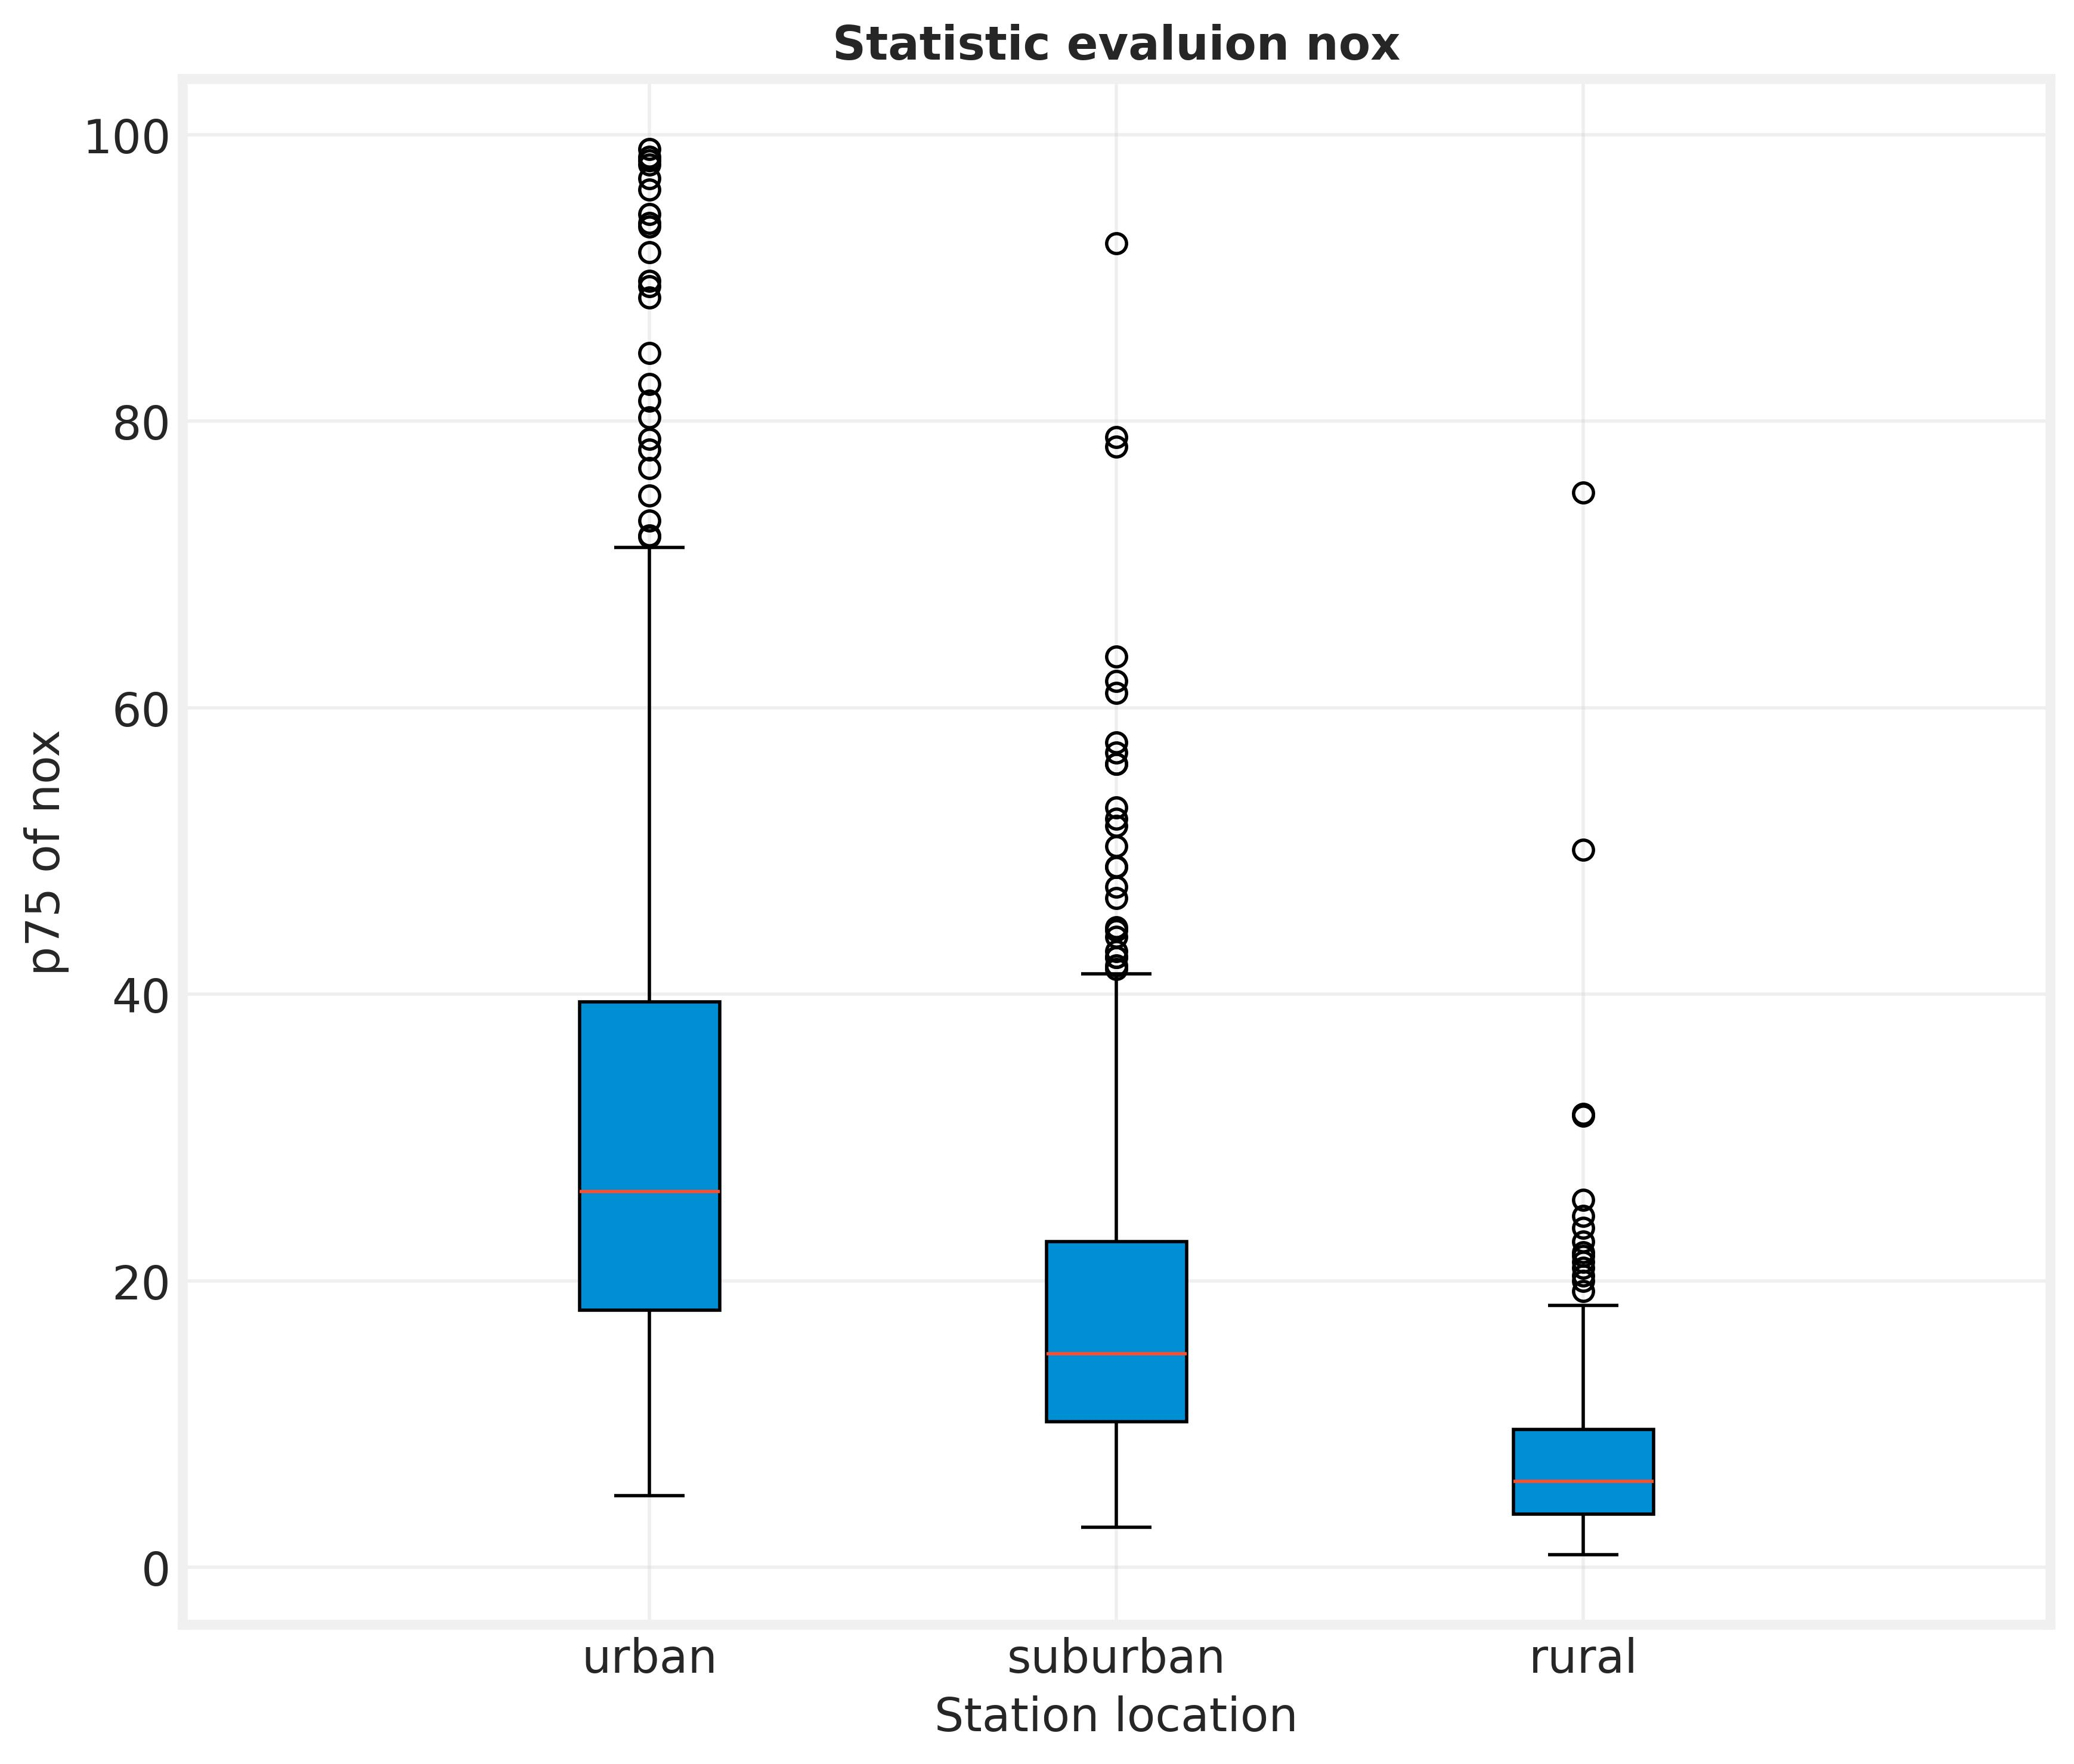
\includegraphics[width=0.45\textwidth]{figures/box_nox.jpg} \label{elbow}} 
    \hskip 0.2cm
    \subfigure[]{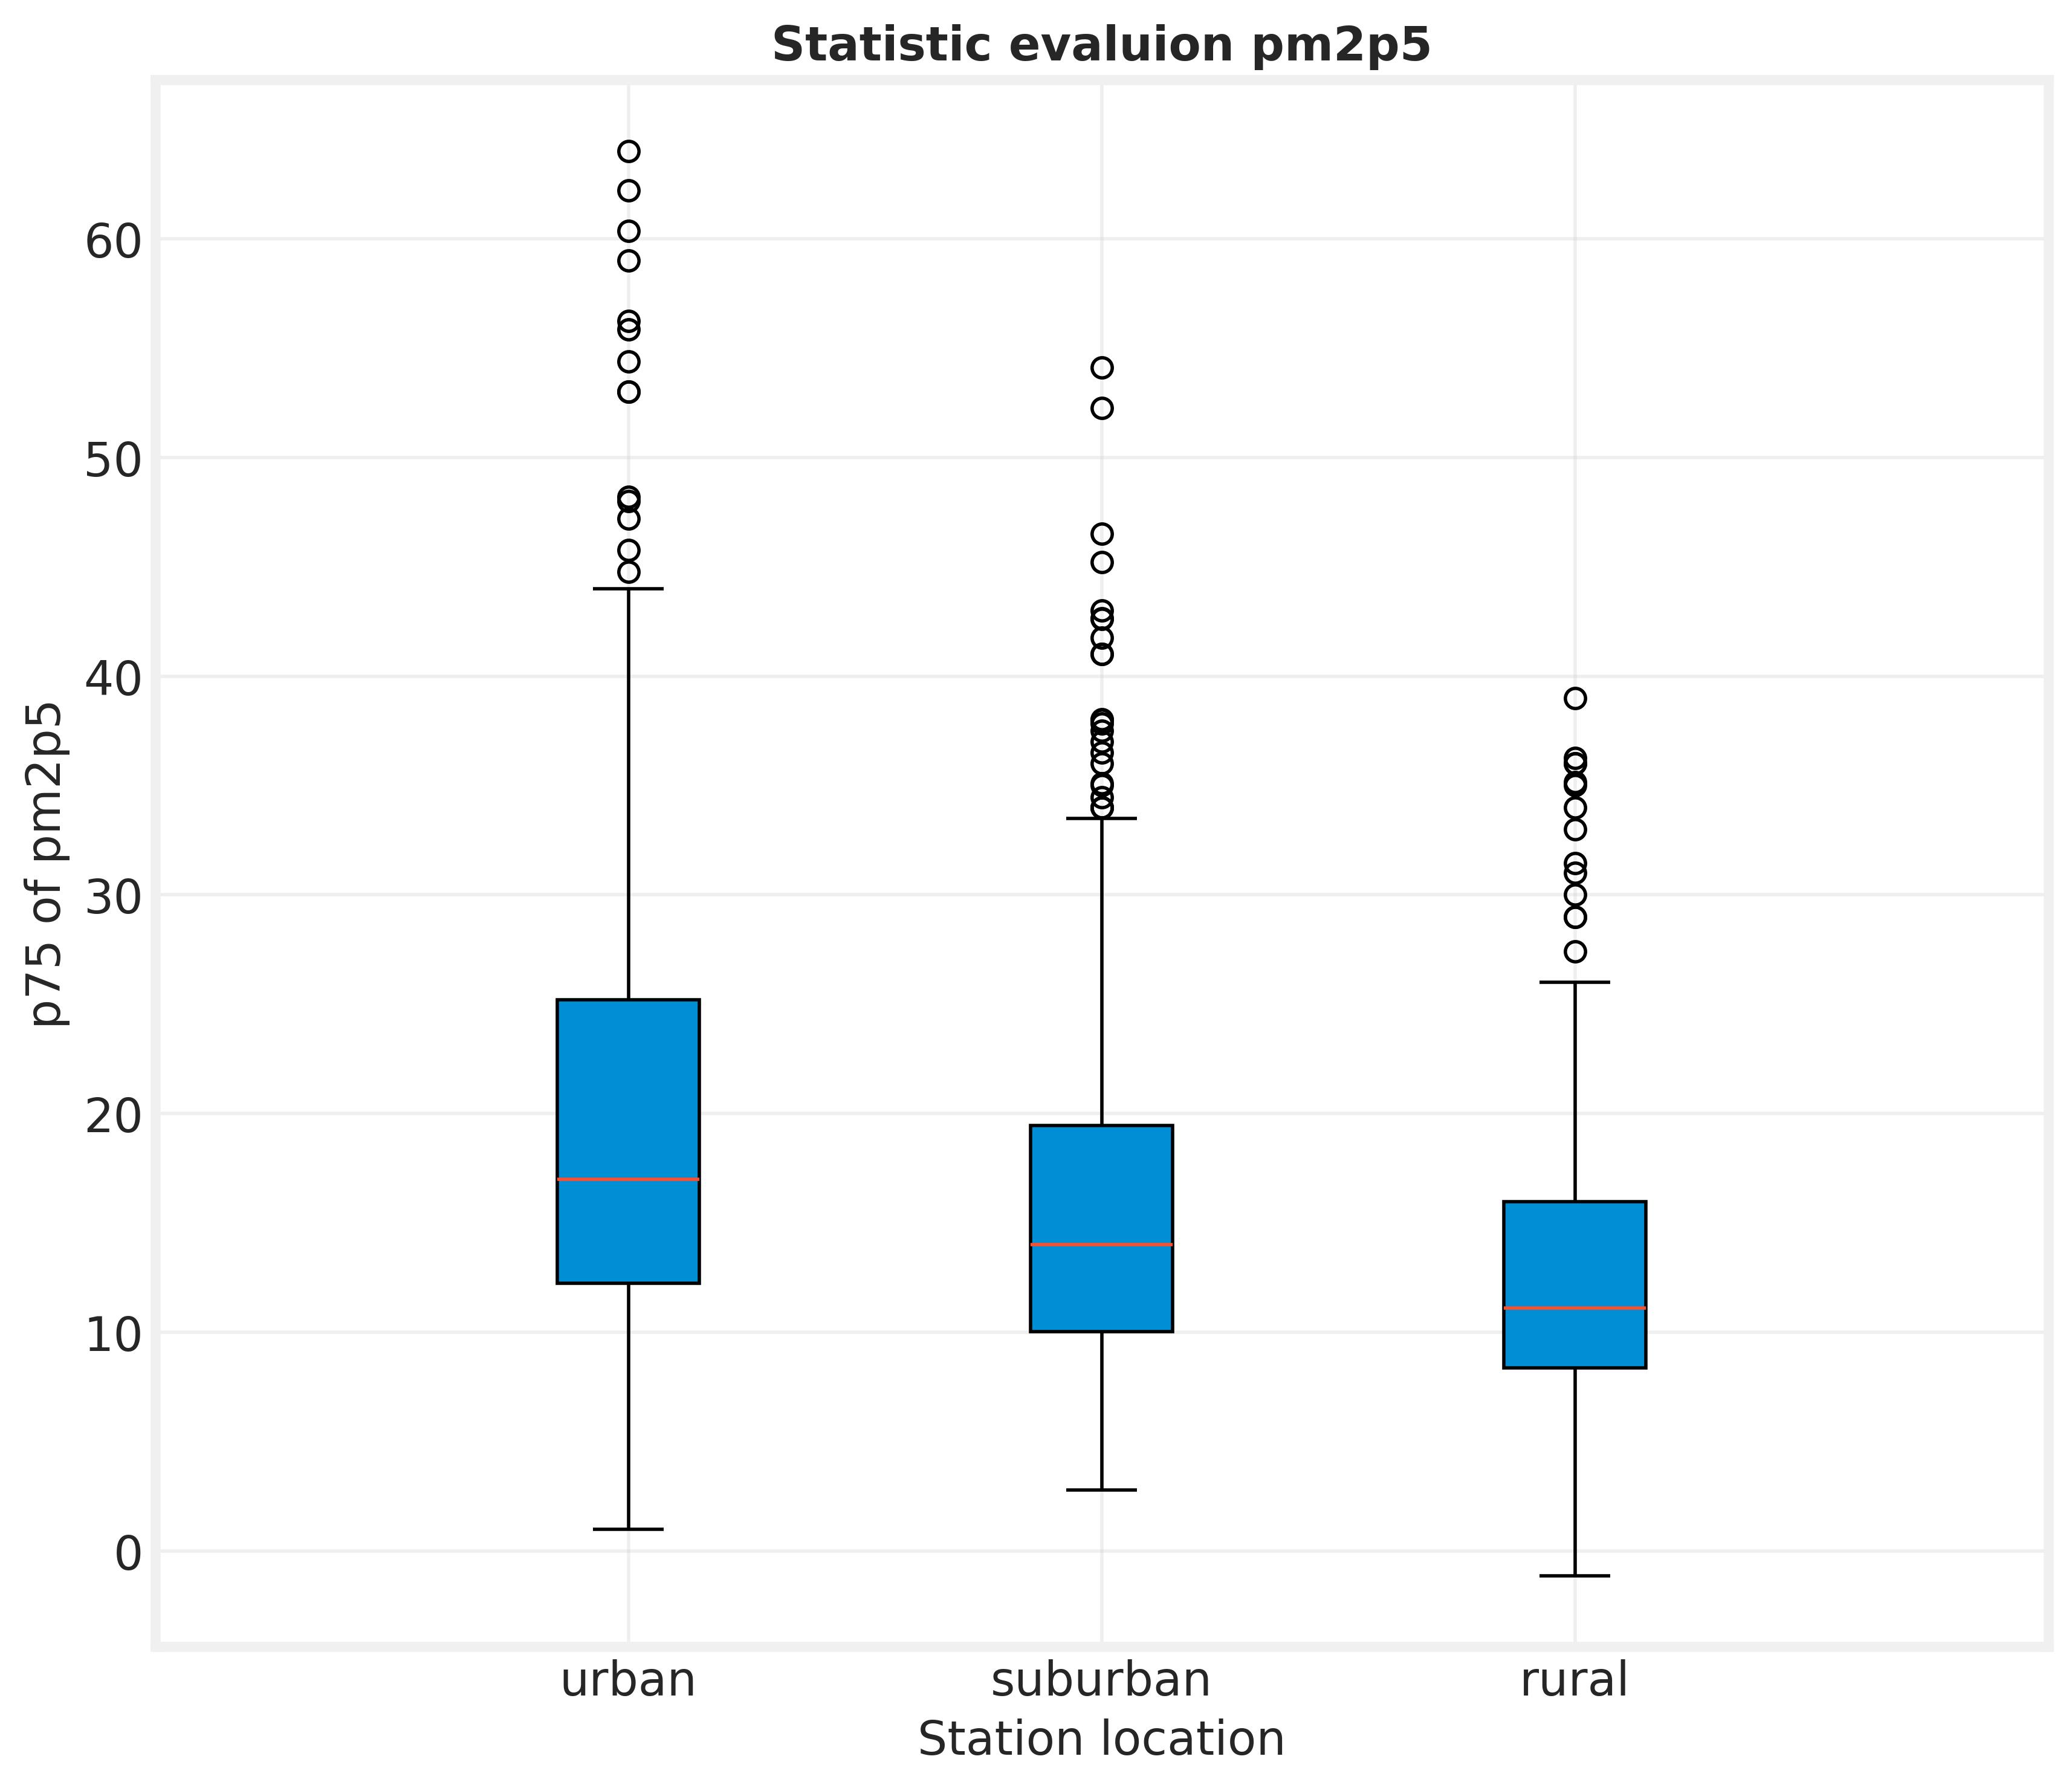
\includegraphics[width=0.45\textwidth]{figures/box_pm2p5.jpg} \label{stat_eval}}
    \caption{Evaluation of the supervised classification with independent data: (a)  Box and whisker plot of the 75 percentile of the NOx. (b) Box and whisker plot 75 percentile of the PM2.5}
    \label{nox_pm_eval}
\end{figure}
\newpage
\section{Conclusion} %% \conclusions[modified heading if necessary]
We investigated the use of machine learning models to objectively characterize station locations for global air quality data analysis. Specifically, we wanted to improve the station classification in the TOAR-I database that was described by \cite{schultz2017tropospheric} and base it on an objective algorithm. As a side-effect we can now explicitly label stations as suburban that were falling between the urban and rural categories in the TOAR-I classification scheme. Our proposed models demonstrate excellent prediction capabilities for urban and rural areas. With the help of an adjusted probability threshold technique, we also obtain meaningful results on the suburban category, inasmuch this category can be described objectively at all. We noticed a limitation for evaluating the accuracy of our method due to obvious misclassification of stations in official databases. As discussed in \citep{schultz2017tropospheric}, such errors can be introduced for various reasons. In some cases, we speculate that these misclassifications actually reflect true landcover changes (e.g., urban development), which have not been updated in the station metadata at the data providers' sites. Manual inspection of random test samples with disagreements revealed that the ML classifier was more often correct than the reported station type.

There is still room for improvement of the methods described here. On the one hand, a larger manual labelling effort using high-resolution EO data, could reduce the number of wrong target labels and reduce the noise in the training data. On the other hand, it may also be possible to employ modern ML methods with spatial context (e.g., \citep{szwarcman2024prithvi}) on such high-resolution EO data directly as a specialized land cover classification task. Nevertheless, the new TOAR station classifiers developed in this study provide a clear improvement over the previous method and can be employed in the TOAR-II ozone data analyses that will be reported in the forthcoming assessment papers.
%% The following commands are for the statements about the availability of data sets and/or software code corresponding to the manuscript.
%% It is strongly recommended to make use of these sections in case data sets and/or software code have been part of your research the article is based on.
%\codedataavailability{}
\newpage
\textbf{Code data availability }\\All code accompanying this paper is available in our GitLab repository  link\citep{Mache2025TOARClassifier} at the following link: \\
\href{https://doi.org/10.5281/zenodo.15411286}{https://doi.org/10.5281/zenodo.15411286}. 
This repository also contains a copy of the data that is used in this sudy as csv files. The data can also be obtained directly from the  \href{https://toar-data.fz-juelich.de/api/v2}{TOAR-II database}. %% use this section when having data sets and software code available

%\sampleavailability{TEXT} %% use this section when having geoscientific samples available

%\videosupplement{TEXT} %% use this section when having video supplements available

% \appendix
% \section{}    %% Appendix A

% \subsection{}     %% Appendix A1, A2, etc.


%\noappendix       %% use this to mark the end of the appendix section. Otherwise the figures might be numbered incorrectly (e.g. 10 instead of 1).
%% Regarding figures and tables in appendices, the following two options are possible depending on your general handling of figures and tables in the manuscript environment:
%% Option 1: If you sorted all figures and tables into the sections of the text, please also sort the appendix figures and appendix tables into the respective appendix sections.
%% They will be correctly named automatically.

%% Option 2: If you put all figures after the reference list, please insert appendix tables and figures after the normal tables and figures.
%% To rename them correctly to A1, A2, etc., please add the following commands in front of them:

%\appendixfigures  %% needs to be added in front of appendix figures

%\appendixtables   %% needs to be added in front of appendix tables

%% Please add \clearpage between each table and/or figure. Further guidelines on figures and tables can be found below.
%\authorcontribution{}
\vspace{0.5cm}

\textbf{Author contribution}\\ RKM, SS, and MGS designed the study based on previous work by MGS and SS. RKM, AP, and ML developed the methodology, RKM implemented the methods and evaluated the results. RKM wrote the major part of the text with contributions from all authors. MGS conducted a final review prior to submission.\vspace{0.5cm}\\%\vspace{1cm} %% this section is mandatory
%\competinginterests{}

\textbf{Competing interests}\\The authors declare that no competing interests exist.\\ %% this section is mandatory even if you declare that no competing interests are present
%\disclaimer{TEXT} %% optional section
%\begin{acknowledgements}

\textbf{Acknowledgements}\\
The authors are grateful to the EU for funding the IntelliAQ project under grant ERC-AdG-787576. This allowed the buildup of the TOAR-II database. We also greatly appreciate the effort from hundreds of people around the world who established and operate air quality stations, process the data and make the data available to the TOAR initiative. Sebastian Hickman deserves gratitude for his initial analysis of NOx and PM2.5 data in the TOAR-II database and helpful discussions.
%\end{acknowledgements}

%Referee suggestion
% Paul Griffiths, paul.griffiths@ncas.ac.uk, The National Centre for Atmospheric Science is a world leading research centre, supported by the Natural Environment Research Council (UK), Cambridge University, URL: https://www.ch.cam.ac.uk/group/atm/person/ptg21
% Gaige Kerr, gaigekerr@email.gwu.edu Milken Institute School of Public Health, https://publichealth.gwu.edu/departments/environmental-and-occupational-health/gaige-kerr
% Mariliza Koukouli , Aristotle University of Thessaloniki, mariliza@auth.gr, https://msc-env.physics.auth.gr/teachers/koukouli-mariliza/?lang=en

%%% Cover letter
% Dear editors,

% please consider our manuscript on a data-driven classification tool for global air quality stations for publication in GMD. In this paper, we describe an objective method to obtain globally consistent labels, i.e. urban, rural, and suburban, for air quality measurement sites. This classification replaces the more subjective method that had been employed in the first Tropospheric Ozone Assessment Report and shall be used in the analysis of data in the ongoing second Tropospheric Ozone Assessment Report.

% Our method builds on a variety of machine learning models including k-means clustering,  Random Forest, CatBoost and  LightGBM. All code and data are made available on a GitLab repository. Once the paper is accepted, we will generate a tar archive from the code including all data and submit this as supplement.

% Kind regards
% Ramiyou Karim Mache
%% REFERENCES

%% The reference list is compiled as follows:


%% Since the Copernicus LaTeX package includes the BibTeX style file copernicus.bst,
%% authors experienced with BibTeX only have to include the following two lines:
%%
%% \bibliographystyle{copernicus}
%% \bibliography{example.bib}
%%
%% URLs and DOIs can be entered in your BibTeX file as:
%%
%% URL = {http://www.xyz.org/~jones/idx_g.htm}
%% DOI = {10.5194/xyz}


%% LITERATURE CITATIONS
%%
%% command                        & example result
%% \citet{jones90}|               & Jones et al. (1990)
%% \citep{jones90}|               & (Jones et al., 1990)
%% \citep{jones90,jones93}|       & (Jones et al., 1990, 1993)
%% \citep[p.~32]{jones90}|        & (Jones et al., 1990, p.~32)
%% \citep[e.g.,][]{jones90}|      & (e.g., Jones et al., 1990)
%% \citep[e.g.,][p.~32]{jones90}| & (e.g., Jones et al., 1990, p.~32)
%% \citeauthor{jones90}|          & Jones et al.
%% \citeyear{jones90}|            & 1990



%% FIGURES

%% When figures and tables are placed at the end of the MS (article in one-column style), please add \clearpage
%% between the bibliography and first table and figure and between each table and figure.

% The figure files should be labeled correctly with Arabic numerals (e.g. fig01.jpg, fig02.png).


%% ONE-COLUMN FIGURES

%%f
%\begin{figure}[t]
%\includegraphics[width=8.3cm]{FILE NAME}
%\caption{TEXT}
%\end{figure}
%
%%% TWO-COLUMN FIGURES
%
%%f
%\begin{figure*}[t]
%\includegraphics[width=12cm]{FILE NAME}
%\caption{TEXT}
%\end{figure*}
%
%
%%% TABLES
%%%
%%% The different columns must be separated with a & command and should
%%% end with \\ to identify the column brake.
%
%%% ONE-COLUMN TABLE
%
%%t
%\begin{table}[t]
%\caption{TEXT}
%\begin{tabular}{column = lcr}
%\tophline
%
%\middlehline
%
%\bottomhline
%\end{tabular}
%\belowtable{} % Table Footnotes
%\end{table}
%
%%% TWO-COLUMN TABLE
%
%%t
%\begin{table*}[t]
%\caption{TEXT}
%\begin{tabular}{column = lcr}
%\tophline
%
%\middlehline
%
%\bottomhline
%\end{tabular}
%\belowtable{} % Table Footnotes
%\end{table*}
%
%%% LANDSCAPE TABLE
%
%%t
%\begin{sidewaystable*}[t]
%\caption{TEXT}
%\begin{tabular}{column = lcr}
%\tophline
%
%\middlehline
%
%\bottomhline
%\end{tabular}
%\belowtable{} % Table Footnotes
%\end{sidewaystable*}
%
%
%%% MATHEMATICAL EXPRESSIONS
%
%%% All papers typeset by Copernicus Publications follow the math typesetting regulations
%%% given by the IUPAC Green Book (IUPAC: Quantities, Units and Symbols in Physical Chemistry,
%%% 2nd Edn., Blackwell Science, available at: http://old.iupac.org/publications/books/gbook/green_book_2ed.pdf, 1993).
%%%
%%% Physical quantities/variables are typeset in italic font (t for time, T for Temperature)
%%% Indices which are not defined are typeset in italic font (x, y, z, a, b, c)
%%% Items/objects which are defined are typeset in roman font (Car A, Car B)
%%% Descriptions/specifications which are defined by itself are typeset in roman font (abs, rel, ref, tot, net, ice)
%%% Abbreviations from 2 letters are typeset in roman font (RH, LAI)
%%% Vectors are identified in bold italic font using \vec{x}
%%% Matrices are identified in bold roman font
%%% Multiplication signs are typeset using the LaTeX commands \times (for vector products, grids, and exponential notations) or \cdot
%%% The character * should not be applied as mutliplication sign
%
%
%%% EQUATIONS
%
%%% Single-row equation
%
%\begin{equation}
%
%\end{equation}
%
%%% Multiline equation
%
%\begin{align}
%& 3 + 5 = 8\\
%& 3 + 5 = 8\\
%& 3 + 5 = 8
%\end{align}
%
%
%%% MATRICES
%
%\begin{matrix}
%x & y & z\\
%x & y & z\\
%x & y & z\\
%\end{matrix}
%
%
%%% ALGORITHM
%
%\begin{algorithm}
%\caption{...}
%\label{a1}
%\begin{algorithmic}
%...
%\end{algorithmic}
%\end{algorithm}
%
%
%%% CHEMICAL FORMULAS AND REACTIONS
%
%%% For formulas embedded in the text, please use \chem{}
%
%%% The reaction environment creates labels including the letter R, i.e. (R1), (R2), etc.
%
%\begin{reaction}
%%% \rightarrow should be used for normal (one-way) chemical reactions
%%% \rightleftharpoons should be used for equilibria
%%% \leftrightarrow should be used for resonance structures
%\end{reaction}
%%% PHYSICAL UNITS
%%%
%%% Please use \unit{} and apply the exponential notation
\clearpage
\bibliographystyle{copernicus}
\bibliography{ref}
\end{document}
